\documentclass{article}
\usepackage{float}
\usepackage{graphicx}
\usepackage{fancyhdr}
\usepackage{geometry}
\usepackage{xcolor, soul}
\usepackage{changepage}  % allows temporary margin adjustments
\usepackage{amsmath}
\usepackage[font=footnotesize, textfont=it, justification=centering]{caption}
\usepackage{subcaption}
\usepackage{wrapfig}
\usepackage{multirow}
\usepackage{booktabs}
\usepackage{amssymb}
\usepackage{soul,xcolor}
\usepackage{pgfplots}
\pgfplotsset{compat=1.18}
\usepackage{siunitx}
\usepackage{url}
\usepackage{ctable}
\usepackage{natbib}
\bibliographystyle{plain}
\usepackage{cleveref}
\usepackage{physics}
\usepackage[inline]{enumitem}
\usepackage{overpic}
\usepackage[normalem]{ulem}
\captionsetup[sub]{textfont=it,font=footnotesize,justification=centering}
\usetikzlibrary{intersections}
\usepgfplotslibrary{fillbetween}

\geometry{margin=2cm}

%Function for skipping lines
\newcommand{\newpara}
    {
    \vskip 1 mm
    \noindent
    }

\setlength{\fboxsep}{0pt} % Padding between border and image
\setlength{\fboxrule}{0.5pt} % Thickness of the border

\title{\textbf{3A1b Full Technical Report - Boundary Layers: \\ Transition to Turbulence}}
\author{
  Fontaine, Noah\\
  \texttt{nf391}
  \and
  Pembroke College\\
  \texttt{March 2026}}
\date{}

\begin{document}

\maketitle

\section{Introduction, Aims and Objectives}

In low-to-moderate Reynolds number flow regimes, the stability of a laminar boundary layer is significantly influenced by external factors such as surface disturbances and acoustic noise. Any instability can trigger an earlier onset of the transition process to turbulent boundary layers. Understanding this process is vital as the transition point serves as a primary determinant for many engineering applications, such as the skin friction and overall efficiency of aerodynamic surfaces of turbine blades and wings \cite{nasa_boundary_layer}.

This experiment investigates the sensitivity of boundary layers to a flat plate and two different flow-altering geometries -- a roughness element (screw) and a tripwire -- in a controlled wind tunnel environment and employing hot-wire anemometry and acoustic detection techniques.

The main aims and objectives of this lab are to:
\begin{itemize}[itemsep=0.1pt]
    \vspace{-6pt}
    \item Determine the transition Reynolds numbers associated with each of the three tested flow configurations and quantify the spanwise angle of the turbulent wedge generated by an isolated roughness element.
    \item Derive estimates for the skin friction coefficient based on the mean velocity profiles, thereby evaluating the impact of flow state on wall shear stress. Find the boundary layer's integral properties including the displacement thickness $\delta^*$, the momentum thickness $\theta$, and the shape factor $H$.
    \item Characterize the turbulent boundary layer profile by fitting it against theoretical canonical profiles and the logarithmic overlap law of the wall.
    \item Investigate the nature of transition or flows with smooth leading edges and the onset of turbulence via the formation of two-dimensional Tollmien-Schlichting waves, Emmons spots and Laminar Separation Bubbles.
    \item Explore the high sensitivity of boundary layers to small surface imperfections and extract practical uses of of this instability to prevent flow separation under adverse pressure gradients.
\end{itemize}

\section{Experimental Methodology}

\subsection{Calibration and Instrumentation}

Before data collection, the hot-wire anemometer probe is calibrated to establish the relationship between the bridge voltage ($E$) and the local flow velocity ($U$). This relationship is governed by King’s Law, expressed as
\begin{equation*}
    E^2 = A + BU^{0.5}
\end{equation*}
where $A$ and $B$ are constants. Once calibrated, the probe allows the local velocity fluctuations $u'$ and 10 \unit{\second} mean flow local velocities $\bar{u}$ to be measured.

\subsection{Transition Observation and Flow Conditions}

To identify the point of transition from purely laminar to fully turbulent flow, the probe is positioned at a constant height of $y=0.5$ \unit{\mm} above the wall. By analyzing the voltage signal and varying the velocity freestream flow, the Reynolds number of the transition stages are identified for three distinct configurations:
\begin{itemize}[itemsep=0.1pt]
    \vspace{-6pt}
    \item \textbf{Smooth plate}: Measurements are conducted without any surface disturbances to establish a baseline for laminar flow development.
    \item \textbf{Roughness Element}: A small obstacle is introduced at the leading edge of the plate.
    \item \textbf{Tripwire}: A tripwire is installed at the leading edge to force an early onset of turbulence.
\end{itemize}
For each configuration, the dynamic pressure is monitored using a pitot tube placed far away from the surface of the plate, to calculate the corresponding Reynolds number at the point of transition.

\subsection{Boundary Layer Profiling}

Lastly, the boundary layer velocity profile is characterized for the tripped flow configuration. By moving the probe vertically from the plate surface into the freestream, the mean velocity and turbulent fluctuations are recorded. This allows the velocity profile of the boundary layer $\frac{\bar{u}}{\bar{U}_{1}}$ as well as its turbulence intensity, the skin friction coefficient $C_f$ of the flow and the friction velocity $U_*$ to be determined, plotted and analyzed.

\section{Results and Discussion}

\begin{center}
    A table of all the symbols used in this lab -- as well as their units and their definitions -- is provided in Appendix \ref{app:symbols}.
\end{center}

\subsection{Observation of transition}

\subsubsection{Flow development with Reynolds Number}
\label{sec: flow development with Reynolds Number}

\begin{figure}[H]
     \centering
     % Row 1
     \begin{subfigure}[b]{0.32\textwidth}
         \centering
         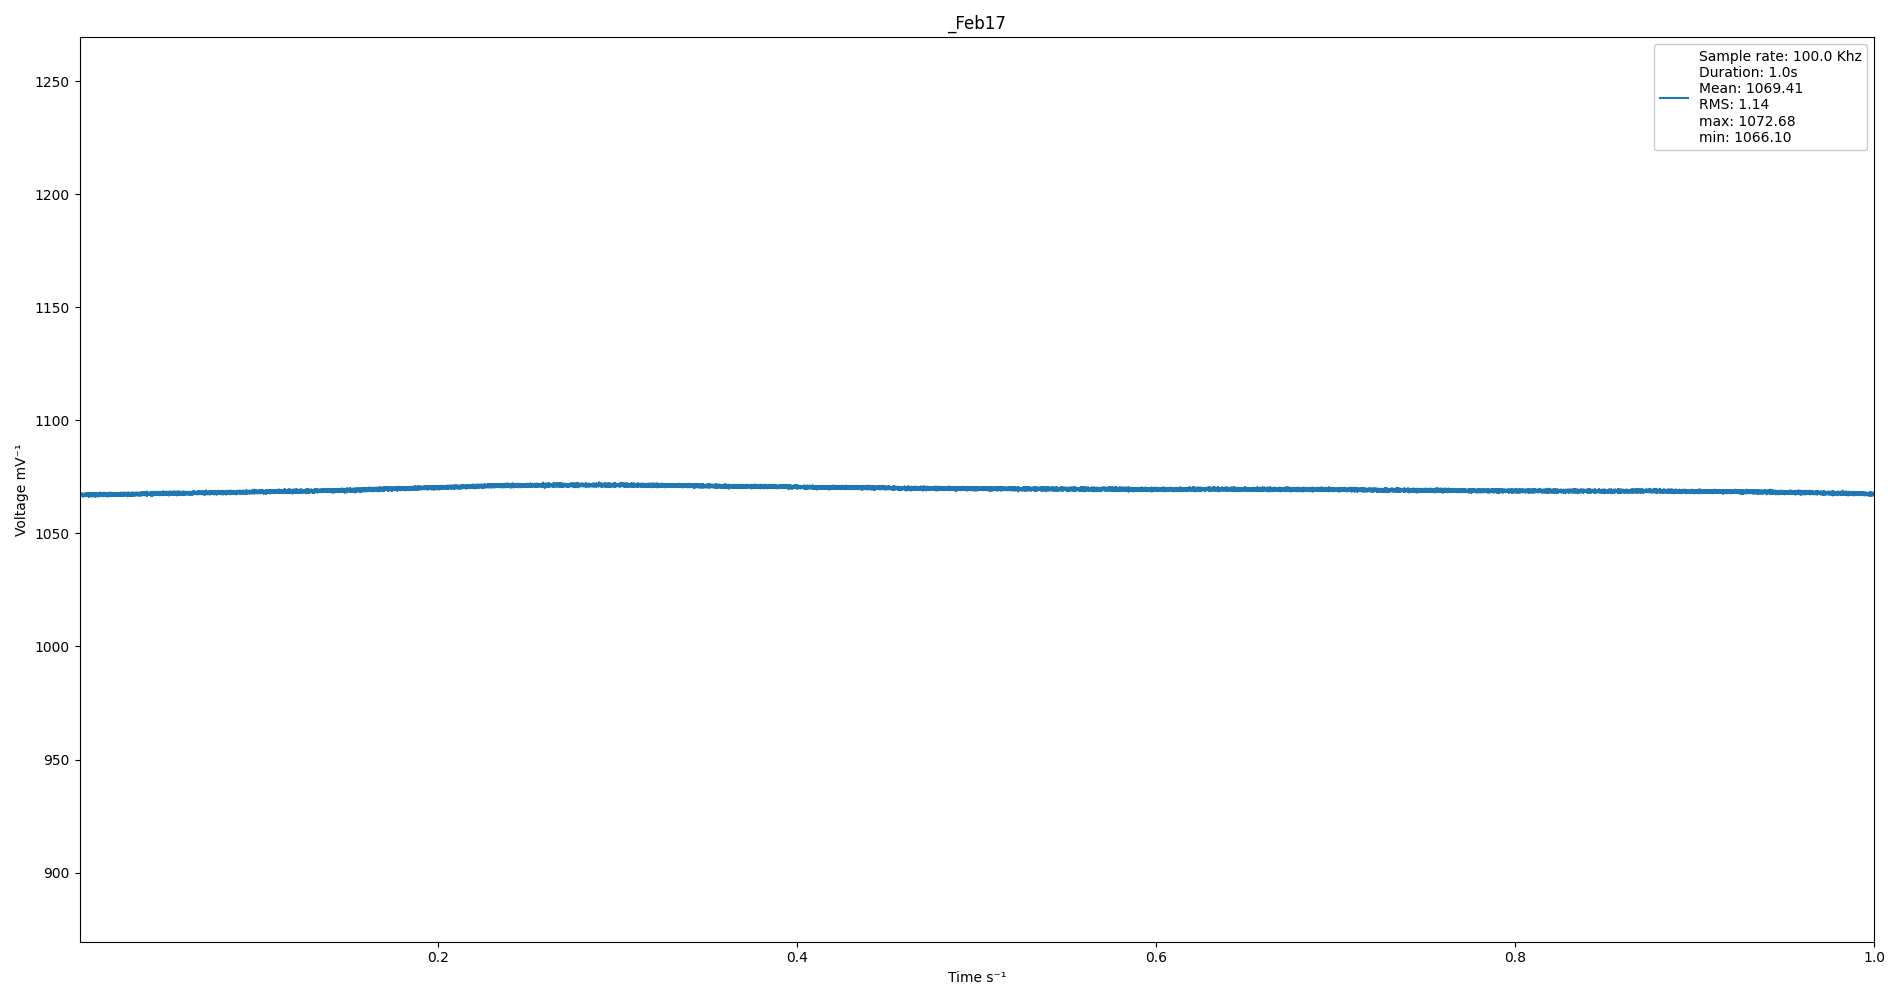
\includegraphics[width=\textwidth]{pictures/smooth_laminar.png}
         \caption{Laminar region on smooth plate.}
         \label{fig:lam smooth}
     \end{subfigure}
     \hfill
     \begin{subfigure}[b]{0.32\textwidth}
         \centering
         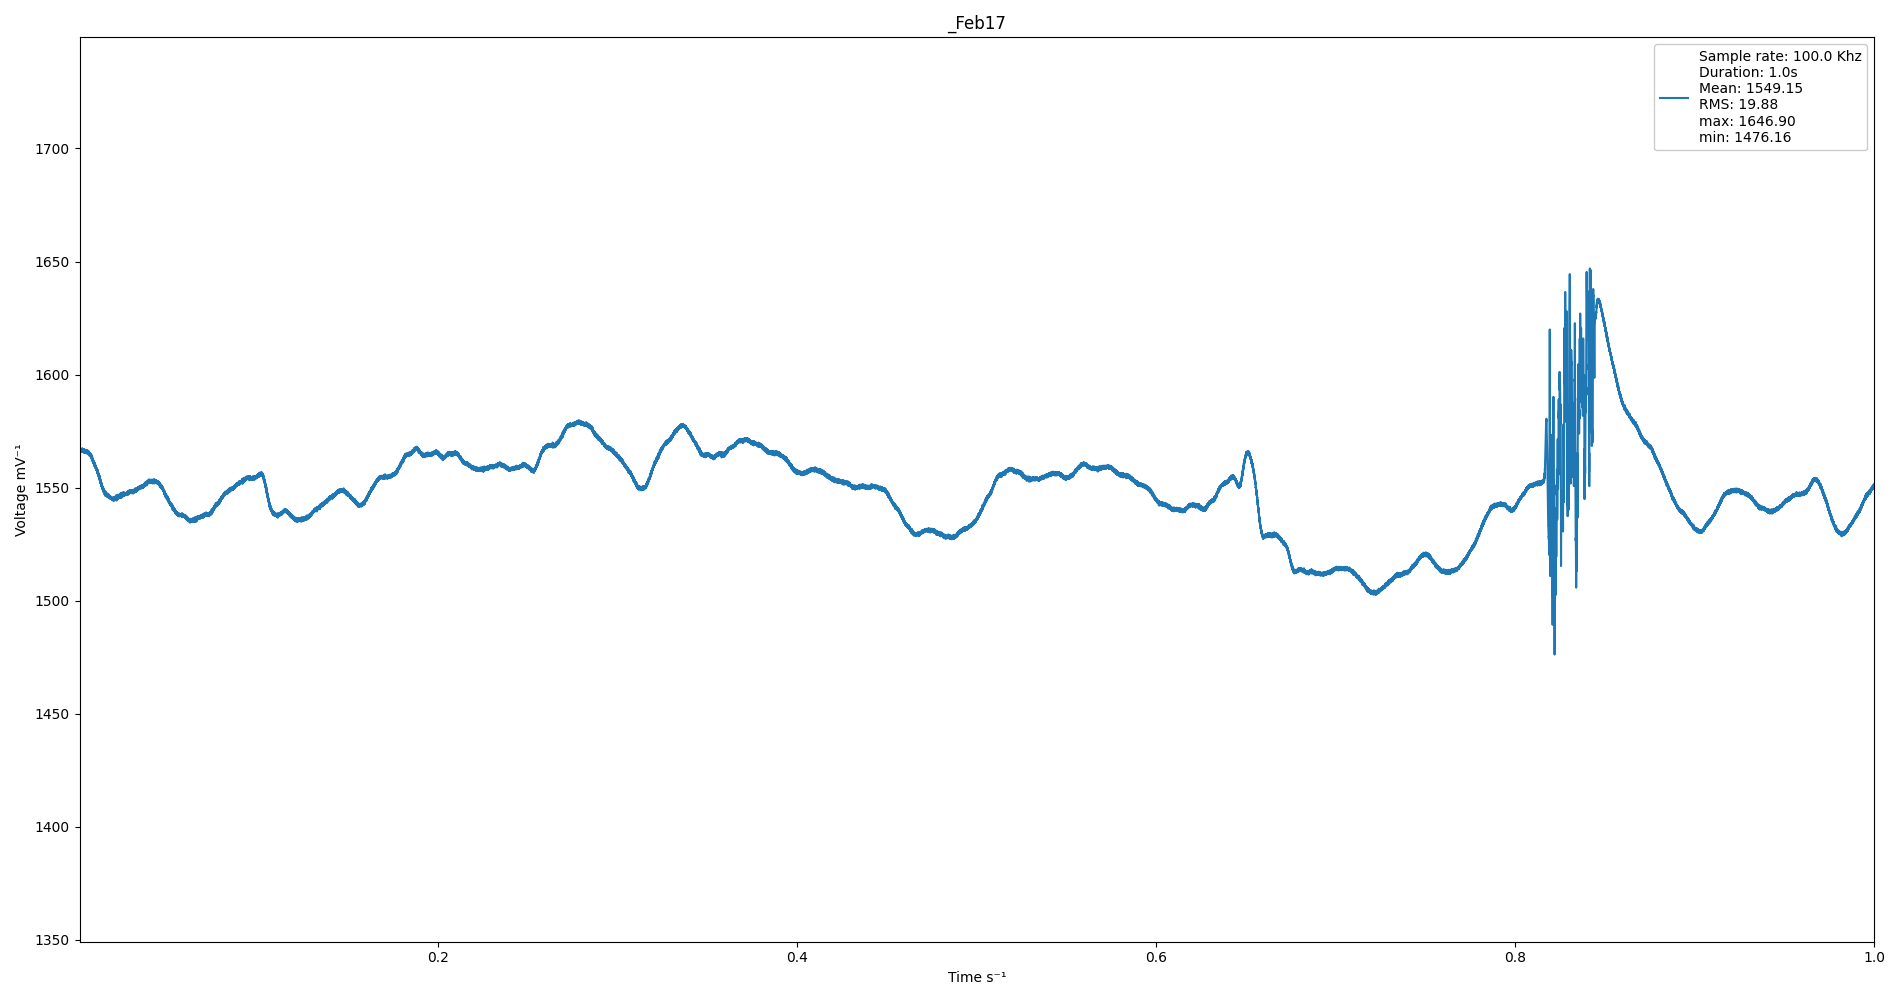
\includegraphics[width=\textwidth]{pictures/smooth_transition.png}
         \caption{Start of turbulence on smooth plate.}
         \label{fig:transition smooth}
     \end{subfigure}
     \hfill
     \begin{subfigure}[b]{0.32\textwidth}
         \centering
         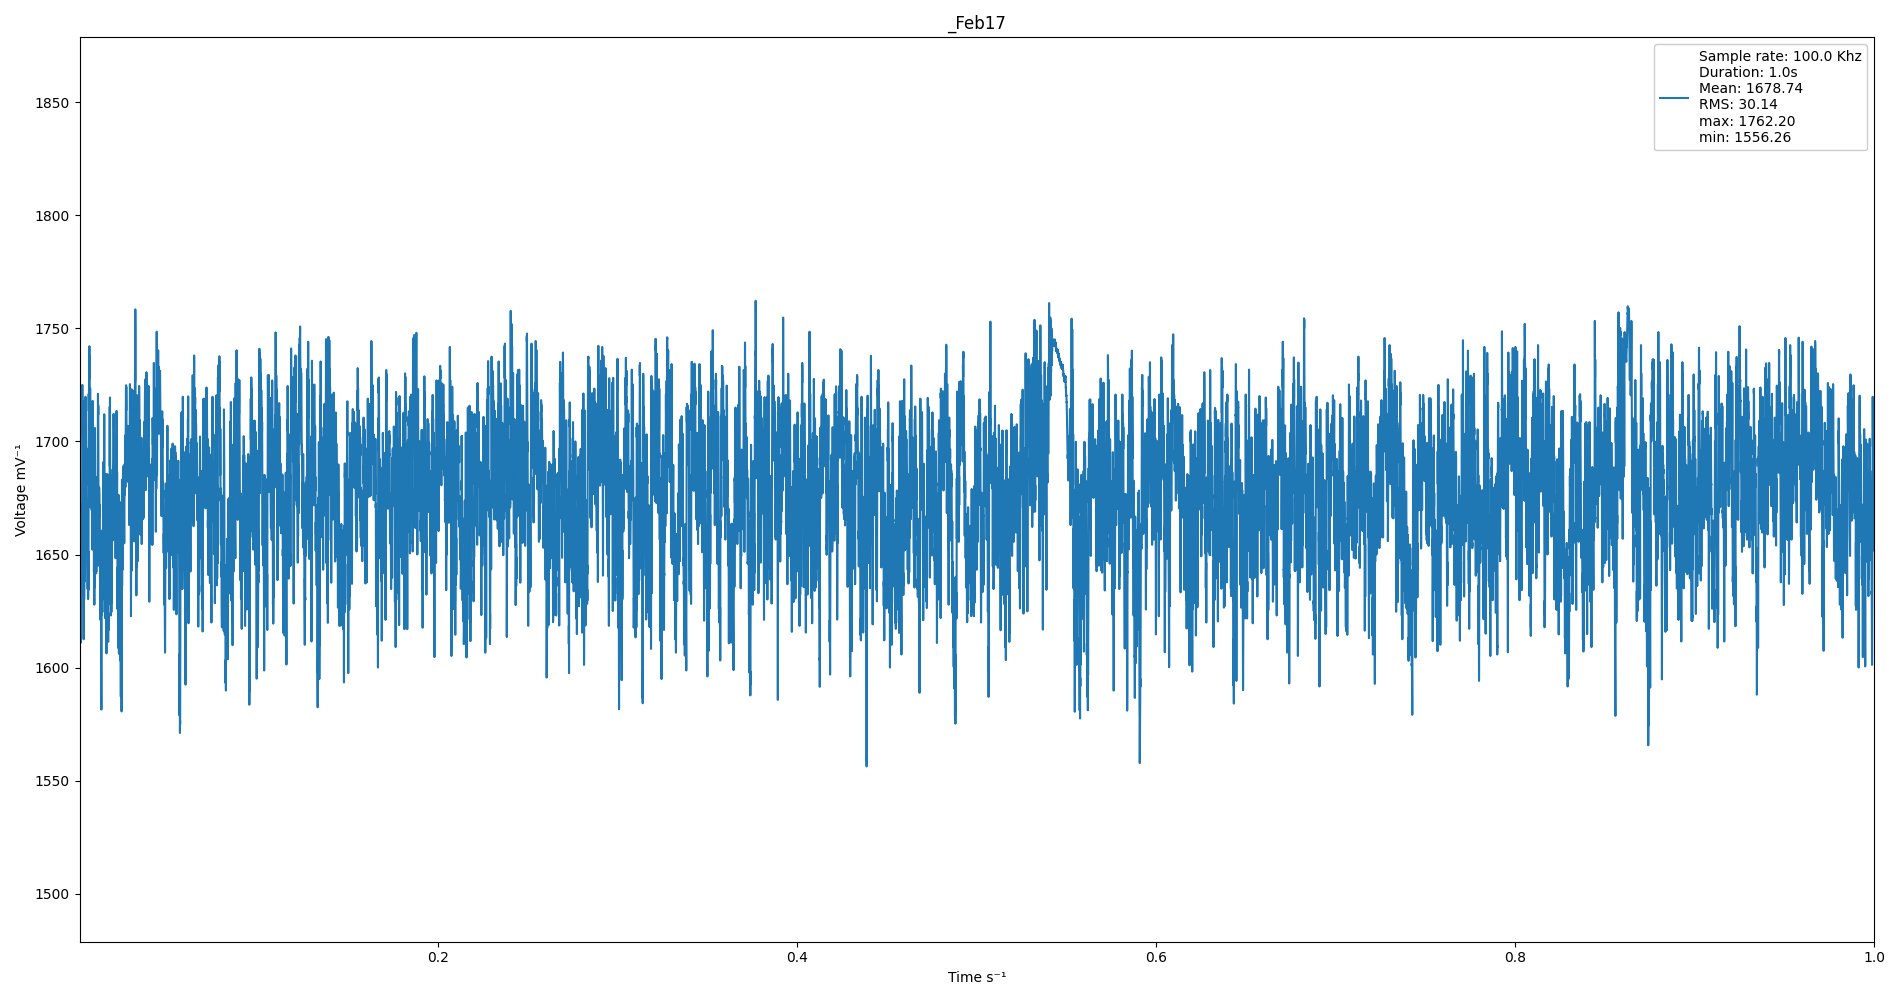
\includegraphics[width=\textwidth]{pictures/smooth_turbulent.png}
         \caption{Fully turbulent region on smooth plate.}
         \label{fig:turbulent smooth}
     \end{subfigure}
     
     \vspace{0.5em} % Add space between rows
     
     % Row 2
     \begin{subfigure}[b]{0.32\textwidth}
         \centering
         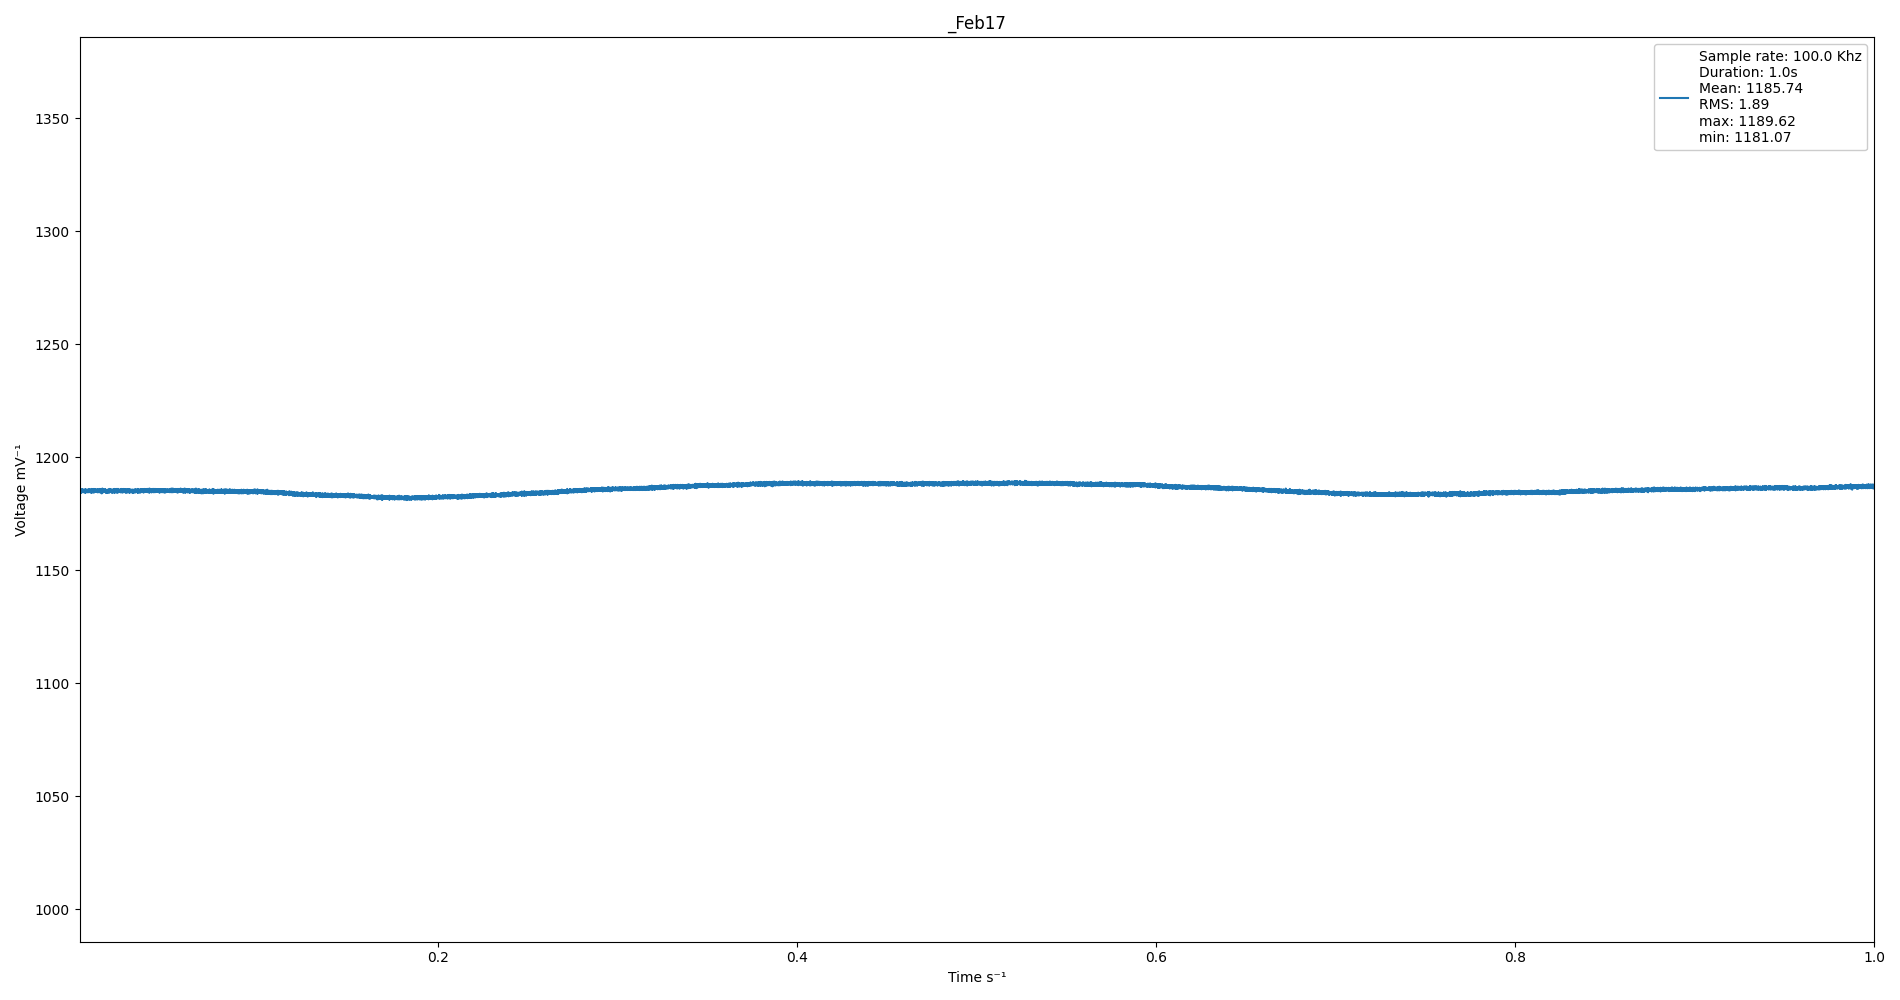
\includegraphics[width=\textwidth]{pictures/roughness_laminar.png}
         \caption{Laminar region with roughness element.}
         \label{fig:lam rough}
     \end{subfigure}
     \hfill
     \begin{subfigure}[b]{0.32\textwidth}
         \centering
         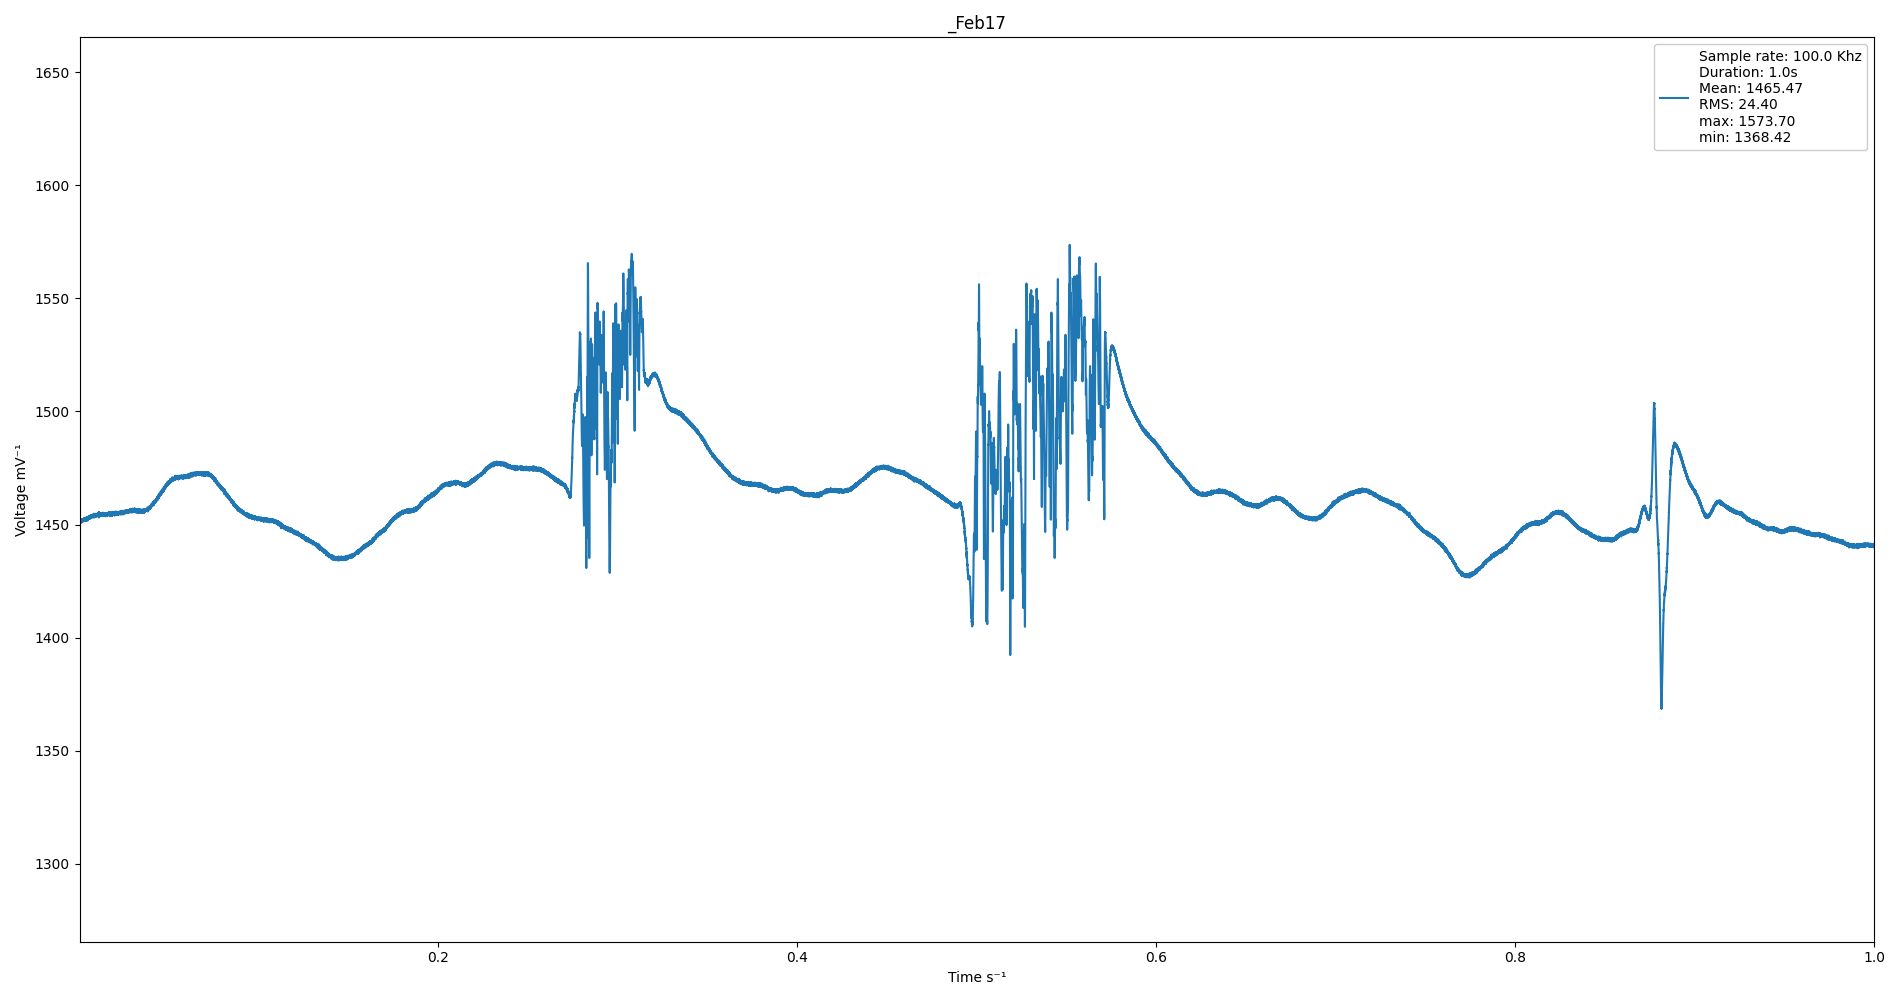
\includegraphics[width=\textwidth]{pictures/roughness_transition.png}
         \caption{Start of turbulence with roughness element.}
         \label{fig:transition rough}
     \end{subfigure}
     \hfill
     \begin{subfigure}[b]{0.32\textwidth}
         \centering
         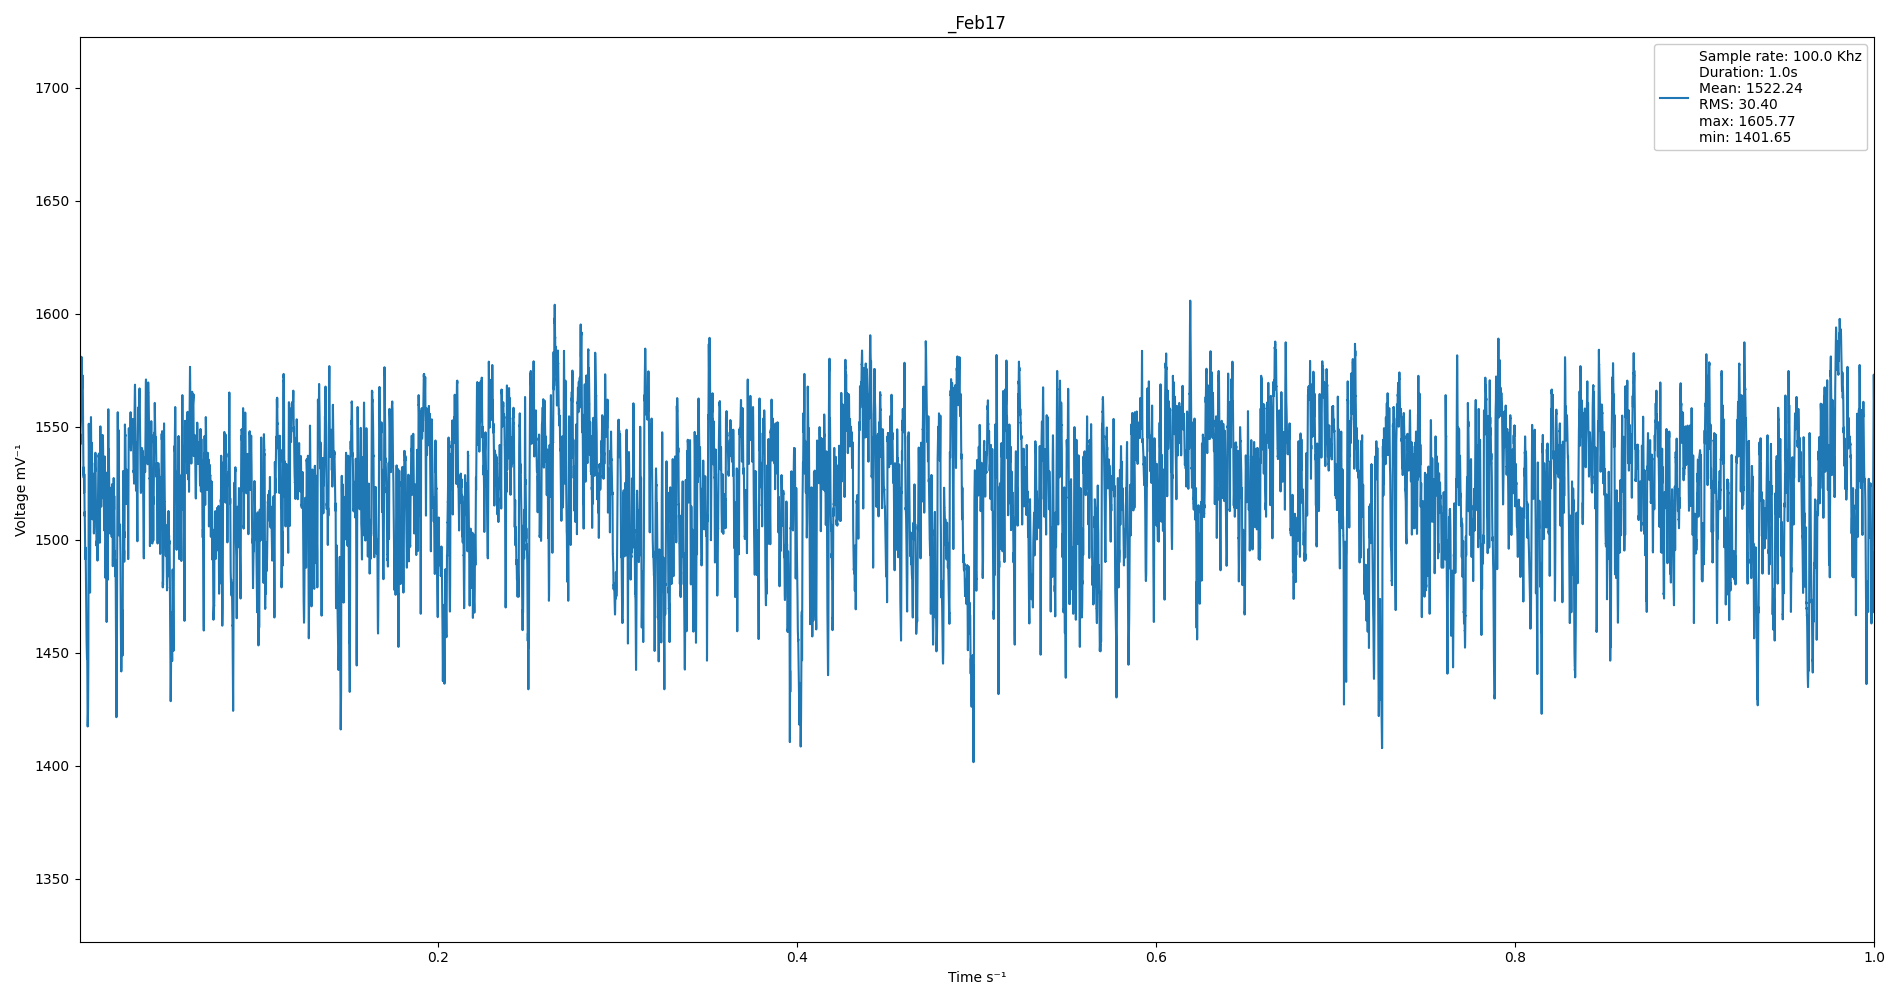
\includegraphics[width=\textwidth]{pictures/roughness_turbulent.png}
         \caption{Fully turbulent region with roughness element.}
         \label{fig:turbulent rough}
     \end{subfigure}
     
     % \vspace{0.5em}
     
     % Row 3
     \begin{subfigure}[b]{0.32\textwidth}
         \centering
         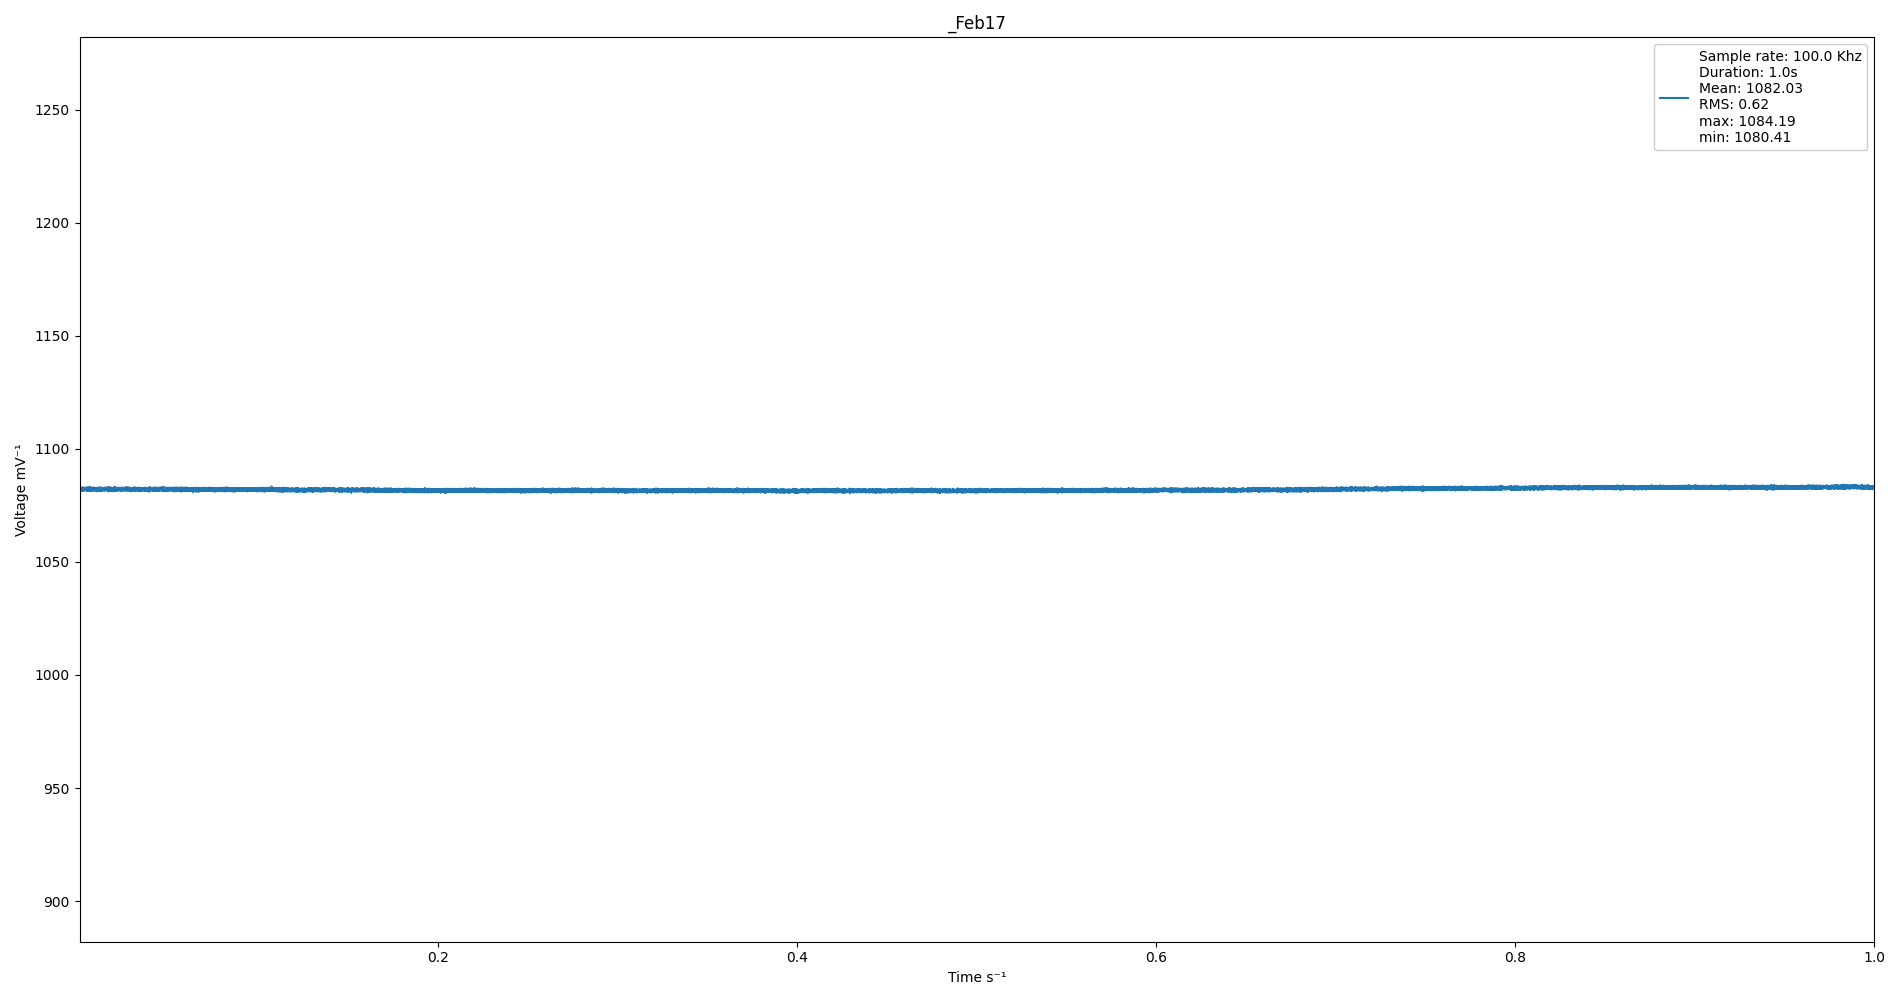
\includegraphics[width=\textwidth]{pictures/tripwire_laminar.png}
         \caption{Laminar region with tripwire.}
         \label{fig:laminar trip}
     \end{subfigure}
     \hfill
     \begin{subfigure}[b]{0.32\textwidth}
         \centering
         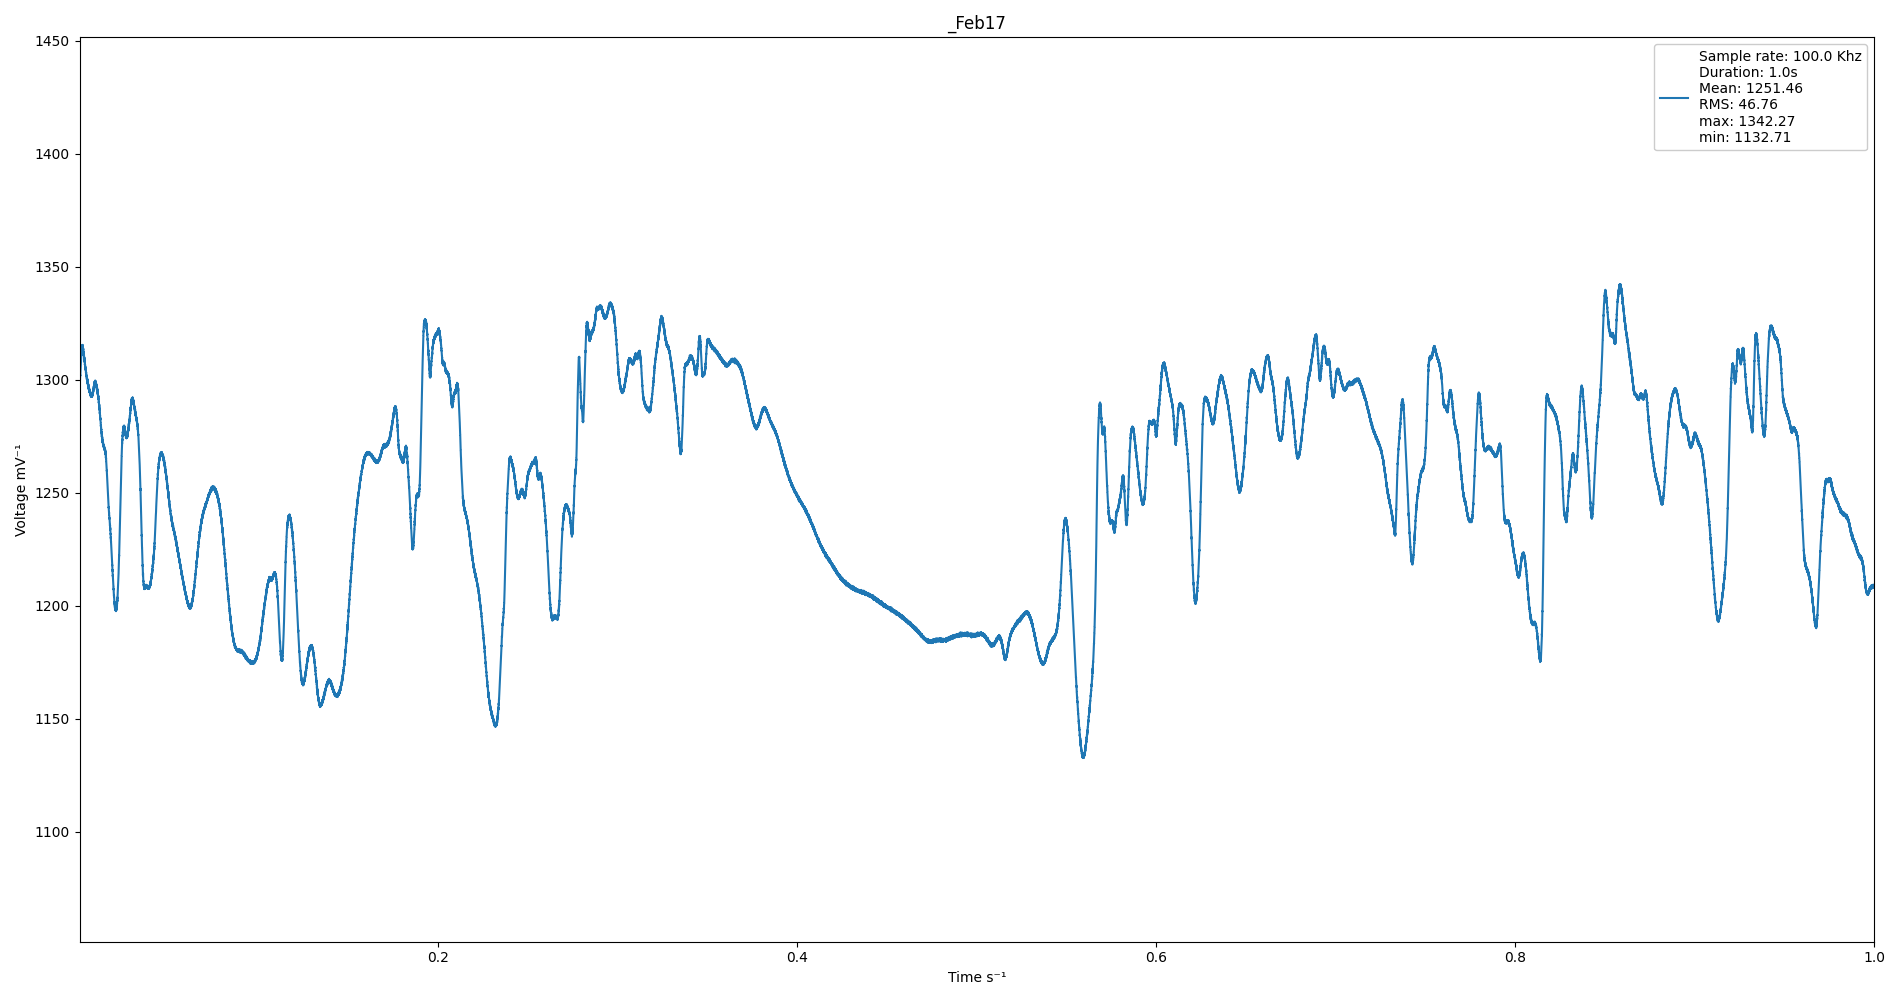
\includegraphics[width=\textwidth]{pictures/tripwire_transition.png}
         \caption{Start of turbulence with tripwire.}
         \label{fig:transition trip}
     \end{subfigure}
     \hfill
     \begin{subfigure}[b]{0.32\textwidth}
         \centering
         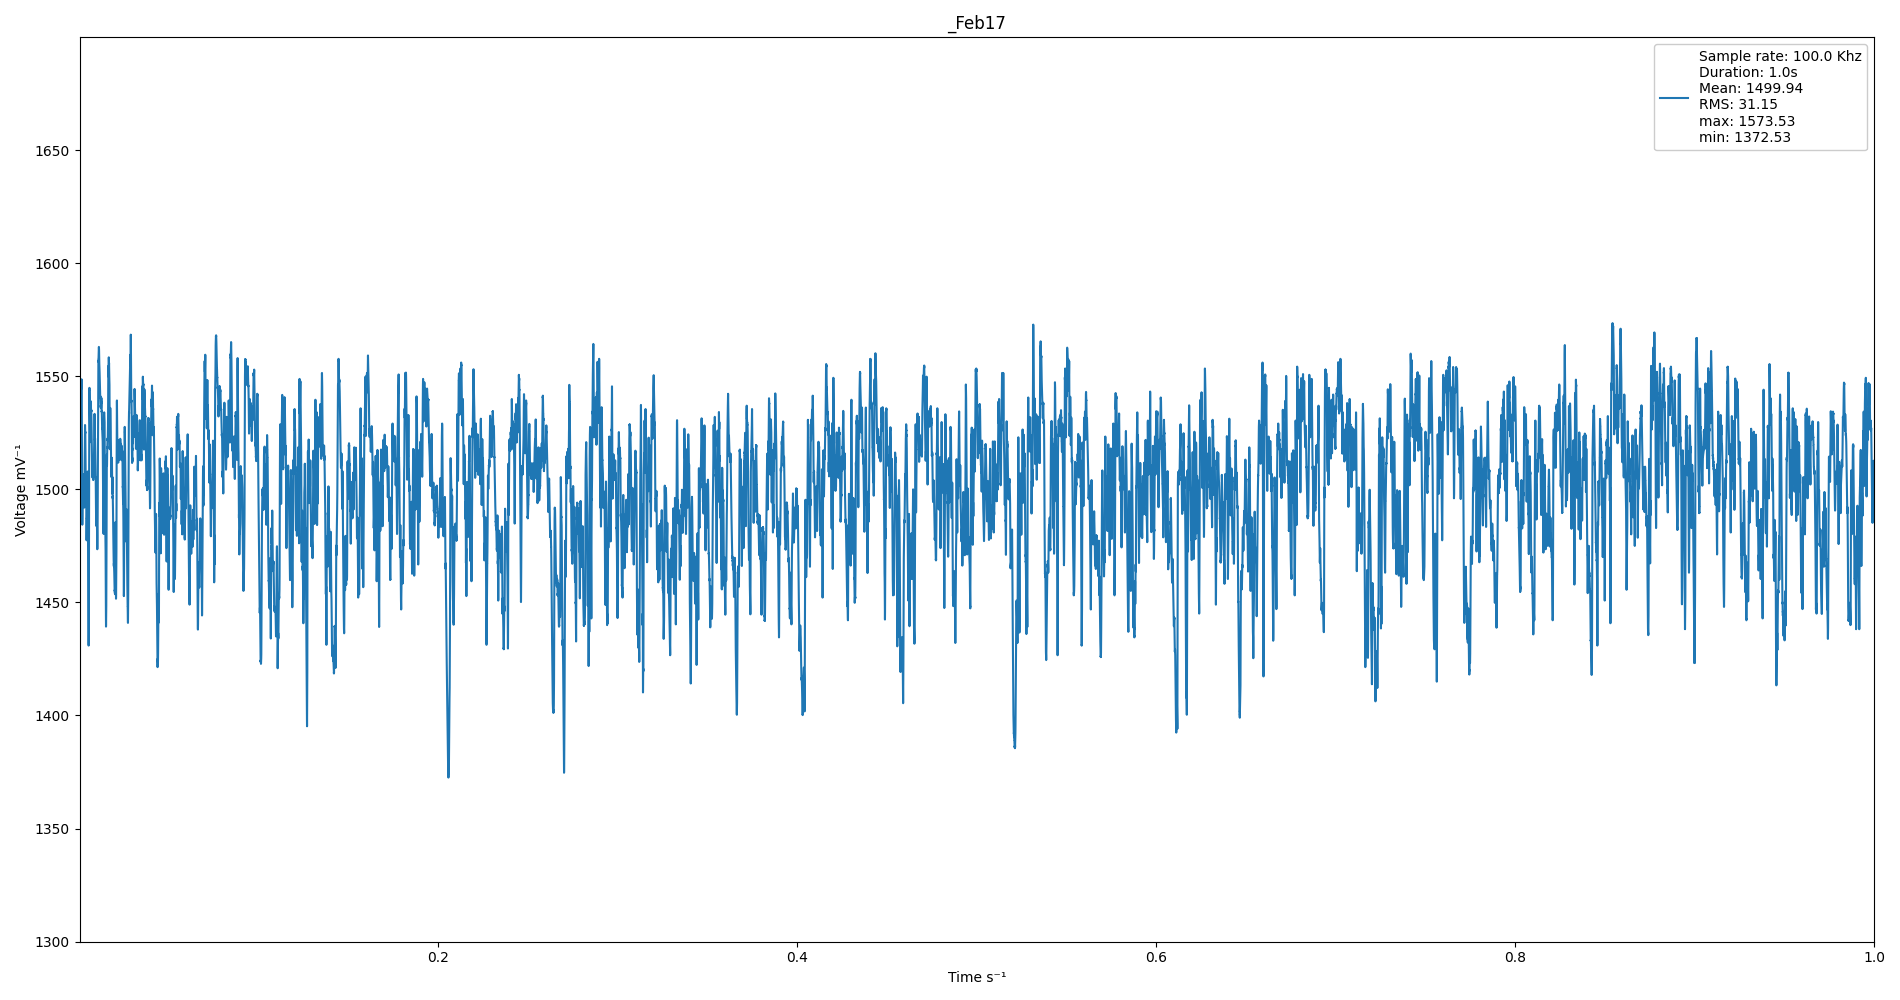
\includegraphics[width=\textwidth]{pictures/tripwire_turbulent.png}
         \caption{Fully turbulent region with tripwire.}
         \label{fig:turbulent trip}
     \end{subfigure}

     \caption{The influence of freestream velocity $\bar{U}_1$ and surface disturbances on boundary layer transition, measured at a wall-normal distance of $y=0.5$ \unit{\mm}.}
     \label{fig:flow development graphs}
\end{figure}

\underline{\bf{NOTE}}: Data and plots for the end of transition region were unfortunately not obtained during the lab. It was very difficult to get qualitative data for the transition region with the tripwire installed, as the transition from fully laminar to fully turbulent flow was very sudden in this configuration.

\Cref{fig:flow development graphs} shows the raw local velocity on a wall-normal distance of $y=0.5$ \unit{\mm}, as measured using the hot wire voltage signals during runs with different surface distributions (smooth plate, roughness element, tripwire) and at different freestream velocities $\bar{U}_1$. At low flow speeds (\ref{fig:lam smooth}, \ref{fig:lam rough}, and \ref{fig:laminar trip}), the flow is laminar and the signal does not have any high frequency components. As the freestream velocity starts to increase, intermittent patches of turbulence start to appear (\ref{fig:transition smooth}, \ref{fig:transition rough}, \ref{fig:transition trip}). These patches are very short, on the order of 50 \unit{\ms}. As the Reynolds number increases further, these turbulent eddies start making up the whole signal, which now contains a lot of high frequency components (\ref{fig:turbulent smooth}, \ref{fig:turbulent rough}, \ref{fig:turbulent trip}).

The values of the Reynolds number at which all these transitions occur is presented in \Cref{fig:turbulent transition}:

\begin{figure}[H]
    \centering
    % \documentclass[margin=3mm]{standalone}
% \usepackage{pgfplots}
\pgfplotsset{compat=1.18}

% \begin{document}
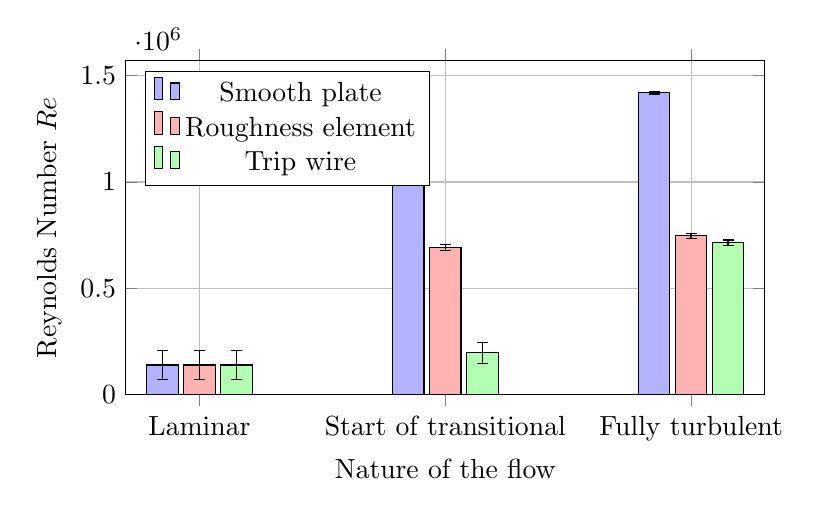
\begin{tikzpicture}
\begin{axis}[
    ybar,
    bar width=0.4cm,           % Adjust width of individual bars
    enlargelimits=0.15,         % Space around the bars
    ylabel={Reynolds Number $Re$},
    xlabel={Nature of the flow},
    symbolic x coords={Laminar, Start of transitional, Fully turbulent},
    xtick=data,
    width=0.8\linewidth,
    height=0.48\linewidth,
    % legend style={at={(0.5,-0.15)}, anchor=north, legend columns=-1},
    legend pos=north west,
    grid=major,
    enlarge y limits={upper=0},
    ymin=0,
]

    % --- 1. Smooth plate ---
    \addplot[
        fill=blue!30,
        error bars/.cd, y dir=both, y explicit,
        error bar style={line width=0.5pt, black}
    ] coordinates {
        (Laminar, 138653.7) +- (0, 69326.8564)
        (Start of transitional, 999846.1) +- (0, 9613.9)
        (Fully turbulent, 1420777.8) +- (0, 6765.6)
    };
    \addlegendentry{Smooth plate}

    % --- 2. Roughness element ---
    \addplot[
        fill=red!30,
        error bars/.cd, y dir=both, y explicit,
        error bar style={line width=0.5pt, black}
    ] coordinates {
        (Laminar, 138653.7) +- (0, 69326.8564)
        (Start of transitional, 693268.6) +- (0, 13865.4)
        (Fully turbulent, 746673.1) +- (0, 12873.7)
    };
    \addlegendentry{Roughness element}

    % --- 3. Trip wire ---
    \addplot[
        fill=green!30,
        error bars/.cd, y dir=both, y explicit,
        error bar style={line width=0.5pt, black}
    ] coordinates {
        (Laminar, 138653.7) +- (0, 69326.8564)
        (Start of transitional, 196086.0) +- (0, 49021.5)
        (Fully turbulent, 713763.7) +- (0, 13467.2)
    };
    \addlegendentry{Trip wire}

\end{axis}
\end{tikzpicture}
% \end{document}
    \caption{Comparison of the calculated Reynolds numbers $Re_x$ at different flow regimes across three distinct experimental conditions: the baseline smooth plate, the surface with a roughness element, and with a tripwire.}
    \label{fig:turbulent transition}
\end{figure}

The roughness element and the tripwire have a huge effect on the value of the Reynolds number at which the flow starts to transition into turbulence, as implied by \Cref{fig:turbulent transition}. Adding either decreases that number from around 1.00 $\times 10^6$ to 6.93 $\times 10^5$ for the roughness element, down all the way to 1.96 $\times 10^5$ for the tripwire. The flow is also fully turbulent much sooner ($Re = 1.42 \times 10^6$ down to $7.47 \times 10^5$ and $7.14 \times 10^5$ respectively), although the nature of the source of turbulence doesn't seem to have a big impact.

It was relatively difficult to access exactly when transition occurred, especially for the tripwire measurements, as these took place at low Reynolds numbers and therefore very low low freestream velocities. The main source of uncertainty regarding Reynolds number calculations came from the precision of the pitot tube which calculates the dynamic head of the freestream flow.

\begin{wrapfigure}[15]{r}{0.48\textwidth}
    \centering
    \vspace{-5em}
    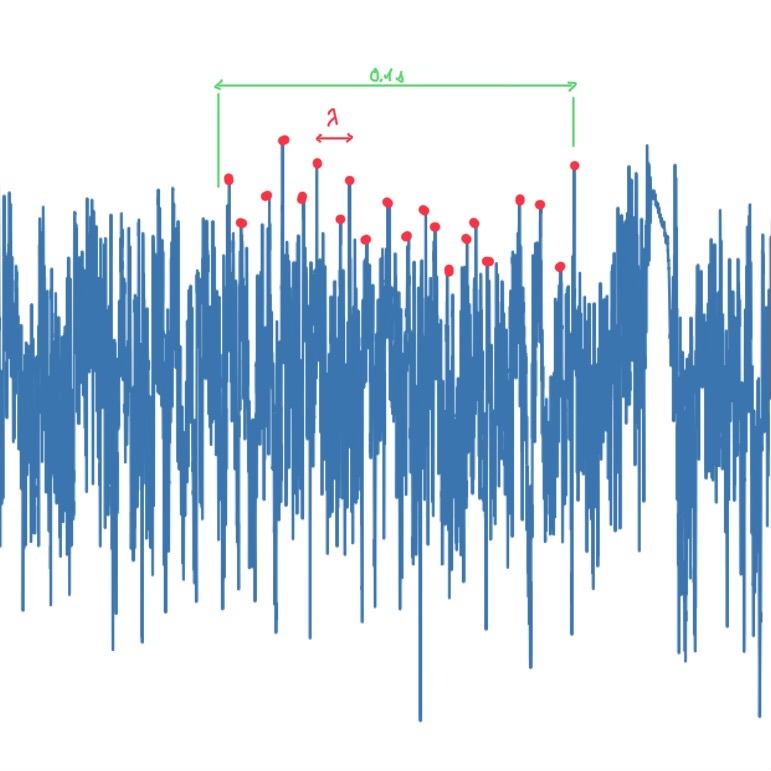
\includegraphics[width=0.92\linewidth]{pictures/eddy_length_2.jpeg}
    \caption{Number of eddies found in 0.1 \unit{\second}}
    \label{fig:eddy}
\end{wrapfigure}

\subsubsection{Turbulent eddy size}

The size of eddies in the turbulent flow was estimated by evaluating their time period in \Cref{fig:flow development graphs}, more specifically \ref{fig:turbulent smooth}. This was found by gauging the time period of as many oscillations as possible $T_N$ (as shown in \Cref{fig:eddy}), dividing by the number of periods $N$ and multiplying by the mean 10 \unit{s} speed of the local flow $\bar{u}$ measured by the probe
\begin{equation}
    \lambda = \frac{T_N}{N} \bar{u}
    \label{eq:eddies}
\end{equation}
\Cref{fig:eddy} shows 20 eddies present in time period of 0.1 \unit{\second}. The freestream mean velocity $\bar{U_1}$ was calculated to be 18.5 \unit{\metre \per \second} (its dynamic head being measured at 2.1 \unit{\milli \bar}). Therefore, from (\ref{eq:eddies}), the average size of a typical eddy in turbulent flow on a smooth plate is around 6.01 \unit{\cm}. This measurement is very approximate and it was difficult to accurately count the number of peaks in the signal analyzed in \Cref{fig:eddy}. Furthermore, due to the stochastic nature of turbulence many more sections would need to be inspected and averaged in order to get an accurate and precise measurement.

\subsubsection{Turbulent wedge profile}
\label{sec:turbulent wedge profile}

\begin{figure}[H]
    \centering
    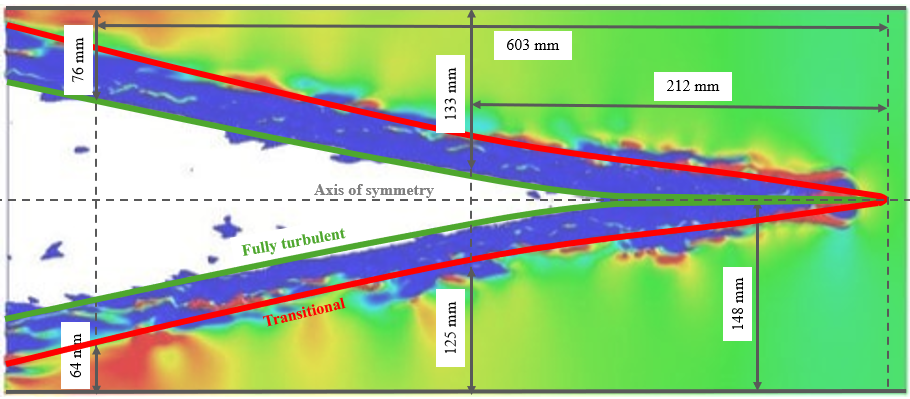
\includegraphics[width=1\linewidth]{pictures/wedges_4.png}
    \caption{Measurement of the transitional and turbulent wakes left by the roughness element (left-running flow). Adapted from \cite{chu2012investigation}.}
    \label{fig:wedge}
\end{figure}

\Cref{fig:wedge} shows the width of the wake left by the roughness element, measured 212 \unit{\mm} and 603 \unit{\mm} behind it. It can be seen that the transition between laminar and turbulent flow is rather sudden as the intermittent 'transitional' zone is quite narrow (0.8 \unit{\mm} and 1.1 \unit{\mm} at the two measurement coordinates). The measurements in \Cref{fig:wedge} imply that the wedge angles $X_{turb}$ and $X_{trans}$ are 8.10 \unit{\degree} and 12.38 \unit{\degree} respectively. What is interesting is that these wedge angles seem to increase the further the wake gets to the roughness element. Indeed, using the measurements taken 603 \unit{\mm} behind, $X_{turb}$ and $X_{trans}$ increase to 13.80 \unit{\degree} and 15.86 \unit{\degree} respectively.

\subsection{Velocity profile}
\label{sec:velocity profile}

\begin{wrapfigure}[19]{r}{0.48\textwidth}
    \centering
    % \documentclass[margin=3mm]{standalone}
% \usepackage{pgfplots}
% \usepackage{siunitx}
% \usepackage{physics}
\usepgfplotslibrary{fillbetween}
\pgfplotsset{compat=1.18}



\begin{tikzpicture}
\begin{axis}[
    xlabel={Velocity profile $\frac{\bar{u}}{\bar{U}_{1}}$},
    ylabel={Distance from surface $y$ [\si{\milli\meter}]},
    major grid style={line width=.2pt,draw=gray!80},
    minor grid style={line width=.1pt,draw=gray!20},
    minor tick num=4,
    xmin=0, xmax=1.1,
    ymin=0,
    grid=both,
    legend pos=north west,
    table/col sep=comma,
]

    % --- 1. Define the Uncertainty Region ---
    % We create two invisible plots to serve as the boundaries
    \addplot[name path=upper, draw=none, forget plot] table [x expr=\thisrow{u_bar_U} + \thisrow{x_error}, y=Dist] {data/velocity_profile.csv};
    \addplot[name path=lower, draw=none, forget plot] table [x expr=\thisrow{u_bar_U} - \thisrow{x_error}, y=Dist] {data/velocity_profile.csv};

    % --- 2. Fill the region ---
    \addplot[blue!10] fill between[of=upper and lower];
    \addlegendentry{$\frac{\bar{u} \pm u'}{\bar{U}_1}$}

    % --- 3. Plot the data points (your scatter plot) ---
    \addplot[only marks, mark=square*, mark size=1pt, blue!70!black] 
        table [x=u_bar_U, y=Dist] {data/velocity_profile.csv};
    \addlegendentry{Mean recorded data}

    % --- 4. Plot your polynomial best fit ---
    \addplot[domain=0.5:20, samples=200, thick, blue, smooth] 
        ({(-0.0009484*x^2 + 0.03746*x + 0.6262)}, {x});
    \addlegendentry{Best fit}

\end{axis}
\end{tikzpicture}
    \caption{Boundary layer velocity profile for a wire-tripped flow at a freestream Reynolds number of $Re_x=9.51\times 10^5$. The velocity is normalized by the freestream velocity $\bar{U}_1$. Shaded region takes into account $u'$, the RMS local velocity.}
    \label{fig:velocity profile}
\end{wrapfigure}

With the tripwire attached to the leading edge of the plate, the 10 \unit{\second} mean of the local velocity $\bar{u}$ and the RMS of the recorded velocity $u'$ were measured at different distances normal to the surface of the plate $y$, and normalized by the freestream mean flow velocity $\bar{U}_1$. This data creates a boundary layer velocity profile that can be seen in \Cref{fig:velocity profile}.

The velocity profile recorded is typical of that found in a turbulent boundary layer -- the initial velocity ratio is very high, which implies a high value of $\dv{\bar{u}}{y}$ and therefore also a high wall shear stress $\tau_w$. This matches the expectation that the recorded flow is fully turbulent ($Re_x=9.51\times 10^5$ which is greater than the $7.14 \times 10^5$ value in \Cref{fig:turbulent transition}). The high shear stress at the wall $\tau_w$ is a result of increased momentum transfer between vertical levels in the boundary layer, due to eddies and vorticity which increase the local velocity closer to the wall and decrease it further from it. This is why turbulent boundary layers are thicker than laminar ones.

Due to the high precision of the micrometer, the error in $y$ is very low and error bars are barely noticeable. Fluctuations in local flow velocity $u'$ seem to stay pretty constant close to the wall (distance $y \lessapprox 15$ \unit{\mm}), but decreases closer to the boundary surface and is essentially null at the surface. This makes sense -- the freestream velocity $U_1$ is constant and the freestream flow is expected to be laminar.

\subsection{Characterization of the turbulent boundary layer profile and its properties}

In order to extract boundary layer properties from the measured velocity profile, including the displacement thickness $\delta^*$, momentum thickness $\theta$, shape factor $H$, and wall shear stress $\tau_w$, the experimental data is first compared against canonical turbulent boundary layer scaling laws. 

In \Cref{sec: canonical profiles} least-squares fits are initially applied to the data to obtain a smooth representation of the velocity profile, which are refined to satisfy the expected boundary conditions at the wall and in the outer flow. They will be ranked according to their correlation of determination coefficients $R^2$. The resulting profile is then assessed against the logarithmic overlap law in \Cref{sec: log law} to evaluate its K\'arm\'an and additive constants.

\subsubsection{Assessment against canonical turbulent boundary layer profiles}
\label{sec: canonical profiles}

The quadratic fit shown in the velocity profile found in \Cref{fig:velocity profile} (equation shown in (\ref{eq:quadratic fit})) has the highest correlation of determination $R^2=0.9971$ out of any simple model, but is not physically accurate. Indeed, it does not fulfill the two necessary boundary conditions.

\begin{enumerate*}[itemjoin={\hspace{16em}}]
    \item $\displaystyle \lim_{y \to 0^+} \bar{u} = 0$
    \item $\displaystyle \lim_{y \to \infty} {\bar{u}} = U_1$
\end{enumerate*}

Two similarity solutions are found that satisfy these boundary conditions. These are non-dimensionalised and put in the form
\begin{equation}
    \eta = f\bigg(\frac{\bar{u}}{U_1}\bigg) \iff \frac{\bar{u}}{U_1} = g(\eta) ; \quad \eta = \frac{y}{\delta} 
\end{equation}
where $\delta$ is the approximate 99\% thickness of the boundary layer. It takes value $\approx 17.22$ \unit{\mm} using the simple quadratic fit found in \Cref{fig:velocity profile}
\begin{equation}
    \eta \approx -9.488 \times 10^{-4} \bigg( \frac{\bar{u}}{U_1} \bigg)^2 + 3.746 \times 10^{-2} \bigg( \frac{\bar{u}}{U_1} \bigg) + 0.6262
    \label{eq:quadratic fit}
\end{equation}
Generally, for turbulent boundary layers on a flat plate with zero pressure gradient, the boundary layer thickness grows with distance using Prandtl's 1/7th Power Law \cite{beltran2019boundarylayerthickness} as
\begin{equation}
    \delta(x) = \frac{0.37 x}{Re_x^{1/5}} \approx 26.89 \hspace{0.4em} \unit{\mm}
    \label{eq:thickness}
\end{equation}
The measured thickness $\delta$ is noticeably smaller than what is expected from (\ref{eq:thickness}), implying that unlike what was assumed in \Cref{sec:turbulent wedge profile}, the boundary layer does not become fully turbulent directly aft of the wedge roughness element. Instead it stays in a laminar or transition region (where $\delta$ is thinner grows more slowly with distance), before full transitioning into the turbulent region. According to \cite{beltran2019boundarylayerthickness} this transition typically occurs at $10^5 \leq Re_x \le 3 \times 10^5$ (in distance terms, $0.12 \le x \le 0.36$ \unit{\metre}). As a reminder, the value of $Re_x$ at the probe where the velocity profile is measured is $\approx 9.51 \times 10^5$ ($x = 1.14$ \unit{\metre}).

The two self-similar solutions that are fitted against the experimental data are an exponential profile and a power law profile (derived from \cite{schlichting1961boundary}). They are in the form:
\begin{enumerate}[noitemsep]
    \item \textbf{Exponential profile}: $\displaystyle \frac{\bar{u}}{U_1} = 1-e^{-B\eta}; \quad B = \text{const} \in \mathbb{R}$
    \item \textbf{Power law profile}: $\displaystyle \frac{\bar{u}}{U_1} = \eta^{1/n}; \quad n = \text{const} \in \mathbb{R_+^*} $
\end{enumerate}
The optimal values of $B$ and $n$ were determined using a linear least squares approach and the Normal Equation
\begin{equation}
    \mathbf{y} = \mathbf{X}\beta \iff \beta^* = (\mathbf{X}^T\mathbf{X})^{-1}\mathbf{X}^T\mathbf{y}
\end{equation}
where $\beta^*$ is the optimal value of either $1/n$ or $-B$. Full derivation is shown in Appendix \ref{app:least squares method}.

\underline{Found solutions are}
\begin{equation}
    \frac{\bar{u}}{U_1} \approx 1-e^{-4.662\eta}; \qquad \frac{\bar{u}}{U_1} \approx \eta^{1/6.399}
    \label{eq:solutions}
\end{equation}

\begin{wrapfigure}{r}{0.48\textwidth}
    \centering
    % \documentclass[margin=3mm]{standalone}
% \usepackage{pgfplots}
% \usepackage{siunitx}
% \usepackage{physics}
\usepgfplotslibrary{fillbetween}
\pgfplotsset{compat=1.18}



\begin{tikzpicture}
\begin{axis}[
    xlabel={Velocity profile $\frac{\bar{u}}{\bar{U}_{1}}$},
    ylabel={Normalized distance $\eta = \frac{y}{\delta}$},
    major grid style={line width=.2pt,draw=gray!80},
    minor grid style={line width=.1pt,draw=gray!20},
    minor tick num=4,
    xmin=0, xmax=1,
    ymin=0.01, ymax=1,
    grid=both,
    legend pos=north west,
    table/col sep=comma,
]
    % --- 1. Define the Uncertainty Region ---
    % We create two invisible plots to serve as the boundaries
    \addplot[name path=upper, draw=none, forget plot] table [x expr=\thisrow{u_bar_U} + \thisrow{x_error}, y expr=\thisrow{Dist}/17.22] {data/velocity_profile.csv};
    \addplot[name path=lower, draw=none, forget plot] table [x expr=\thisrow{u_bar_U} - \thisrow{x_error}, y expr=\thisrow{Dist}/17.22] {data/velocity_profile.csv};

    % --- 2. Fill the region ---
    \addplot[black!10] fill between[of=upper and lower];
    \addlegendentry{$\frac{\bar{u} \pm u'}{\bar{U}_1}$}

    % --- 3. Plot the data points (your scatter plot) ---
    \addplot[only marks, mark=square*, mark size=1pt, black!70!black] 
        table [x=u_bar_U, y expr=\thisrow{Dist}/17.22] {data/velocity_profile.csv};
    \addlegendentry{Mean recorded data}

    % --- 4. Plot your polynomial best fit ---
    \addplot[domain=0:1, samples=200, very thick, purple, smooth] 
        ({(1-exp(-4.6624*x))}, {x});
    \addlegendentry{Exponential Profile}

    % --- 4. Plot your polynomial best fit ---
    \addplot[domain=0:1, samples=200, very thick, blue, dashed, smooth] 
        ({(x^(1/7))}, {x});
    \addlegendentry{1/7$^{\text{th}}$ Power Law Profile}

    % --- 4. Plot your polynomial best fit ---
    \addplot[domain=0:1, samples=200, very thick, blue, smooth] 
        ({(x^(1/6.399))}, {x});
    \addlegendentry{Power Law Profile}


\end{axis}
\end{tikzpicture}
    \caption{Different boundary layer velocity profile trend fits. Exponential Profile and Power Law Profile are the functions listed in (\ref{eq:solutions}). Freestream Reynolds number is $Re_x = 9.51 \times 10^5$.}
    \label{fig:velocity fits}
\end{wrapfigure}

The power law profile has a correlation coefficient of $R^2 \approx 0.986$, which is very good. Furthermore, the calculated value of $n \approx 6.399$ is close to the widely accepted empirical value of $n=7$ for zero pressure gradient turbulent boundary layers in the $10^5 \le Re_x \le 10^7$ range (found in \cite{schlichting1961boundary}). Consequentially the experimental results match the 1/7th power law values closely ($R^2 \approx 0.9673)$. From \Cref{fig:velocity fits} the biggest deviations between the Power Law fit and the measured data occurs in the transition between the outer layer and the overlap region (at $\eta \approx 0.35$), but both the outer law profiles and the wall layers closely match. This suggests that the Power Law approximation performs reliably both when viscous or turbulent shear dominate.

The exponential profile has a lower $R^2$ value of $\approx 0.923$. From \Cref{fig:velocity fits} it does not seem to accurately model the speed closer to the wall ($\eta \le 0.3$), especially in the overlap region where viscous shear starts to become important and in the viscous wall sub-layer region where viscous shear dominates. The model could be made much more accurate by removing weightings in the outer layer of the boundary layer ($\eta \gtrapprox 0.4$). There could thus be 2 different models that combine together -- one that approximates the flow where viscous shear is involved (overlap and wall layer), the other where turbulent shear dominates (outer layer).

\subsubsection{Integral thicknesses and shape factor}

Assuming self-similarity, the integral thicknesses of the experimental boundary layer and the two fits were evaluated to further quantify the nature of the velocity profile. The displacement thickness $\delta^*$, momentum thickness $\theta$, and the resulting shape factor $H$ were defined as:
\begin{align}
    \delta^* &= \int_{0}^{\infty} \left( 1 - \frac{\bar{u}}{U_{1}} \right) dy \approx \sum_{i=1}^{n} \frac{1}{2} \left[ \left( 1 - \frac{u_{i}}{U_{1}} \right) + \left( 1 - \frac{u_{i+1}}{U_{1}} \right) \right] \Delta y_{i} \label{eq:displacement thickness}\\
    \theta &= \int_{0}^{\infty} \frac{\bar{u}}{U_{1}} \left( 1 - \frac{\bar{u}}{U_{1}} \right) dy
    \approx \sum_{i=1}^{n} \frac{1}{2} \left[ \frac{u_i}{U_{1}} \left( 1 - \frac{u_i}{U_{1}} \right) + \frac{u_{i+1}}{U_{1}} \left( 1 - \frac{u_{i+1}}{U_{1}} \right) \right] \Delta y_i \label{eq:momentum thickness} \\
    H &= \frac{\delta^*}{\theta}
    \label{eq:shape_factor}
\end{align}

They were found to be:

\begin{table}[htbp]
\centering
\begin{tabular}{lccc}
\toprule
\textbf{Parameter} & \textbf{Experimental} & \textbf{Power Law} ($n \approx 6.4$) & \textbf{Exponential} ($k \approx 4.66$) \\
\midrule
$\delta^*$ (mm) & 2.6645 & 2.3273 & 3.6588 \\
$\theta$ (mm)       & 1.8851 & 1.7731 & 1.8121 \\
Shape factor $H$                       & 1.4134 & 1.3125 & 2.0191 \\
\bottomrule
\end{tabular}
\caption{Boundary Layer Integral Parameters for Experimental and Theoretical Models.}
\label{tab:shape_factor_etc}
\end{table}

Fully developed turbulent boundary layers with no pressure gradients typically have shape factor values $H\approx 1.3-1.5$ \cite{schlichting1961boundary}. The calculated values of $1.4134$ and $1.3125$ for the experimental data and for the power law fit strongly verify this and suggest that the boundary layer is fully turbulent. This is further supported by the high Reynolds number of $9.51 \times 10^5$.

The exponential fit has a shape factor of $H=2.0191$. This is much higher than expected and would indicate a strong adverse pressure gradient as it is close to the turbulent separation value of $H \approx 2.2-2.4$. Clearly it is a very poor fit of the experimental data.

\subsubsection{Skin friction and wall shear stress}
\label{sec: skin friction and wall shear stress}

\begin{figure}[H]
    \centering
    \begin{overpic}[width=0.9\textwidth]{pictures/Clauser_plot.jpg}
        
        % Y-axis label (rotated)
        \put(-4, 20) {\rotatebox{90}{Velocity Ratio $\bar{u}/\bar{U}_{1}$}}
        
        % X-axis label
        \put(50, -1.5) {\makebox(0,0){$y\bar{U}_1/\nu$}}
        
    \end{overpic}
    \vspace{1em}
    \caption{Clauser plot analysis of the boundary layer velocity profile. The fit of the experimental data to the law of the wall suggests a skin friction coefficient of $C_f\approx0.004$.}
    \label{fig:Clauser}
\end{figure}

\Cref{fig:Clauser} suggests a skin friction coefficient $C_f\approx0.004$. This value allows for the determination of the friction velocity, $U_{*}$, according to the following relation (taken from \cite{handout})

\begin{align}
\label{eq:friction velocity}
    U_* &= \bigg( \frac{\tau_w}{\rho} \bigg)^{0.5} = \bigg[ \frac{1}{2} C_f \bar{U}_1^2\bigg]^{0.5} \\
    \implies \quad U_* &= 0.554 \hspace{0.4em} \unit{\metre \per \second} \nonumber
\end{align}

The friction velocity $U_*$ is calculated to be approximately 0.554 \unit{\m \per \s}, corresponding to around 4.5\% of the freestream velocity $\bar{U}_1$, which is not a lot. Physically, this parameter serves as a characteristic velocity scale that quantifies the wall shear stress experienced within the boundary layer from friction with the surface. The wall shear stress $\tau_w$ for turbulent flow on the smooth plate was then solved for using the definition of $U_*$ in (\ref{eq:friction velocity}). It was found to be 0.376 \unit{\pascal}, which is only 15\% higher than the value of 0.320 \unit{\pascal} listed in \cite{fluid_mechanicsfrankwhite} for turbulent flow over a flat plate at $U_1= 12$ \unit{\metre \per \second} and $Re_x = 10^6$.

Interestingly, in \Cref{fig:Clauser}, in the logarithmic overlap layer, the experimental data does not deviate at all from a single $C_f$ curve on the Clauser plot. This implies that there was no pressure gradient. A pressure gradient would affect the slope of the curve in that linear region, making it deviate from any single $C_f$ curve. Due to the growth of boundary layers on the walls of the wind-tunnel and the reduction in freestream area, there is a small expected favorable pressure gradient, which would in theory have for effect to increase the slope of the linear region.

Furthermore, being so close to the wall the measuring probe can skew the velocity measurements slightly and make it look like the friction is different throughout the linear region.

From \Cref{fig:Clauser} and \Cref{fig:log_law}, it is clear that the viscous wall sublayer and the outer layer have an effect on the overlap layer. There is a sort of buffer area in the region $ 7.5 \le y^+ \le 20$, where the data is slightly affected by the linear law $u^+=y^+$. Likewise, the data starts deviating for $y^+ \ge 325$, right before the outer layer region. This is due to the wake term in Coles' law (see \Cref{sec: log law} and (\ref{eq:Coles' wake law})) and would allow any pressure gradients to be easily qunatified.

\subsubsection{Logarithmic overlap law of the wall}
\label{sec: log law}

The turbulent boundary layer is further characterized through comparison with the logarithmic law of the wall, which usually provides more successful and widely validated descriptions of the mean velocity profile in turbulent flows. The measured velocity profile in \Cref{sec:velocity profile}, using the value of the friction velocity $U_*$ estimated in \Cref{sec: skin friction and wall shear stress}, can be expressed in terms of $u^+ = u/U_*$ and $y^+ = y U_* / \nu$. In the overlap layer, $u^+$ and $y^+$ are related by 
\begin{equation}
    u^+ = \frac{1}{\kappa}\ln(y^+) + B
    \label{eq:log law}
\end{equation}
Plotting that data in \Cref{fig:log_law} allows the adherence to the logarithmic overlap law of the wall to be assessed, and the profile characterized by finding the K\'arm\'an and additive constants $\kappa$ and $B$.

\begin{figure}[H]
    \centering
    % \documentclass[margin=3mm]{standalone}
% \usepackage{pgfplots}
% \usepackage{siunitx}
% \usepackage{physics}
\usepgfplotslibrary{fillbetween}
\pgfplotsset{compat=1.18}



\begin{tikzpicture}
\begin{axis}[
    xlabel={$y^+ = \frac{yU_*}{\nu}$},
    ylabel={$u^+ = \frac{\bar{u}}{U_*}$},
    major grid style={line width=.2pt,draw=gray!80},
    minor grid style={line width=.1pt,draw=gray!20},
    minor tick num=4,
    width=0.8\linewidth,
    height=0.48\linewidth,
    xmode=log,
    xmin=3, xmax=2000,
    ymin=0, ymax=25,
    grid=both,
    legend pos=south east,
    table/col sep=comma,
]
    % --- 1. Define the Uncertainty Region ---
    % We create two invisible plots to serve as the boundaries
    \addplot[name path=upper, draw=none, forget plot] table [x=y_plus, y expr=\thisrow{u_plus} + \thisrow{x_error}] {data/log_law.csv};
    \addplot[name path=lower, draw=none, forget plot] table [x=y_plus, y expr=\thisrow{u_plus} - \thisrow{x_error}] {data/log_law.csv};

    % --- 2. Fill the region ---
    \addplot[blue!10] fill between[of=upper and lower];
    % \addlegendentry{$\frac{\bar{u} \pm u'}{\bar{U}_1}$}

    % --- 3. Plot the data points (your scatter plot) ---
    \addplot[only marks, mark=x, mark size=4pt, blue!70!black] 
        table [x=y_plus, y=u_plus] {data/log_law.csv};
    \addlegendentry{Mean recorded data}

    % --- 4. Plot the viscous region ---
    \addplot[domain=1:20, samples=200, thick, blue, smooth] 
        ({x}, {x});

    % --- 4. Plot overlap region ---
    \addplot[domain=7:1000, samples=200, thick, blue, smooth] 
        ({x}, {1.9645*ln(x)+7.5914});


    % \draw [gray, line width=2pt] (axis cs:350, 0) -- (axis cs:350, 25);
    \draw [purple, dashed, line width=1pt] (axis cs:350, 0) -- (axis cs:350, 25);
    \draw [purple, dashed, line width=1pt] (axis cs:20, 0) -- (axis cs:20, 13.2);
    \draw [purple, dashed, line width=1pt] (axis cs:7.5, 0) -- (axis cs:7.5, 7.5);

    \node [anchor=south west, color=black] at (axis cs:13.5, 20) 
    {\small $u^+=y^+$};
    \node [anchor=south west, color=black, rotate=17] at (axis cs:30, 15) 
    {\small $u^+=\frac{1}{0.509}\ln(y^+) + 7.591$};
    \node [anchor=south west, color=purple!80!black] at (axis cs:30, 5) 
    {Logarithmic overlap layer};
    \node [anchor=south west, color=purple!80!black] at (axis cs:3, 0) 
    {Viscous wall layer};
    \node [anchor=south west, color=purple!80!black] at (axis cs:500, 5) 
    {Outer layer};
    % \node [anchor=south west, color=gray!30!black] at (axis cs:100, 10) 
    % {Inner layer};


\end{axis}
\end{tikzpicture}
    \caption{Boundary layer profile plotted on a logarithmic curve to verify the law of the wall for $Re_x = 9.51 \times 10^5$. All measurements seem to be taken in the overlap and outer layers.}
    \label{fig:log_law}
\end{figure}

From \Cref{fig:log_law} it was found using a least-squares fit that $\kappa \approx 0.509$ and $B \approx 7.591$. This is in reasonable agreement with the standard values $\kappa \approx 0.41$ and $B \approx 5.0$ for a flat plate. Any discrepancies can potentially be explained by the surface roughness of the plate.

It is very difficult to measure the profile closer than 0.5 \unit{\mm} from the plate. Therefore, no clear linear viscous sublayer ($u^+ = y^+$) was observed at low $y^+$. The recorded data primarily captures the logarithmic overlap layer and the outer region of the boundary layer, where the behaviour starts deviating from the log-law due to wake effects and pressure gradients. In \Cref{fig:log_law} this deviation starts happening at $y^+ \approx 350$. This value depends on the Reynolds number of the flow. All the data being recorded in the overlap and outer layers indicates that turbulent shear is very much important in these regions and that viscous shear can be neglected in the fitting models in \Cref{sec: canonical profiles}. It is only in the viscous wall layer that viscous shear dominates (in \Cref{fig:log_law} when $y^+ \lessapprox 7$).

The logarithmic model can be improved at the edge of the overlap layer and in the outer region of the boundary layer where turbulent shear dominates by considering Coles' Law of the Wake. This would allow almost 90\% of the profile to be modeled as opposed to the viscous and overlap layers which only account for roughly the first 20\% of the profile. \Cref{eq:log law} is corrected by adding the by adding a wake term
\begin{equation}
    u^{+} = \underbrace{\frac{1}{\kappa} \ln\left(y^{+}\right) + B}_{\text{Log Law}}
    + \underbrace{\frac{2\Pi}{\kappa} \sin^{2}\left(\frac{\pi y}{2\delta}\right)}_{\text{Wake Term}}
    \label{eq:Coles' wake law}
\end{equation}
The wake parameter $\Pi$ captures the small hump seen in \Cref{fig:log_law} at $y^+ \ge 350$ due to wake. This part of the flow is very sensitive to pressure gradients and would allow any adverse or favorable pressure gradients to be quantified, as adverse pressure gradients make $\Pi$ increase.

\subsubsection{Turbulence intensity}

The relative intensity of velocity fluctuations $u'$ can be found by normalizing it against the local 10 \unit{\second} mean velocity $\bar{u}$ (as shown in \ref{fig:boundary_layer_freestream})or the friction velocity $\bar{U}_*$ (as shown in \ref{fig:boundary_layer_friction}).

\begin{figure}[H]
    \centering
    % First image
    \begin{subfigure}[b]{0.49\textwidth}
        \centering
        % \documentclass[margin=3mm]{standalone}
% \usepackage{pgfplots}
% \usepackage{siunitx}
% \usepackage{physics}
\usepgfplotslibrary{fillbetween}
\pgfplotsset{compat=1.18}



\begin{tikzpicture}
\begin{axis}[
    xlabel={Turbulence intensity $\sqrt{\frac{\bar{u}'^2}{\bar{u}^2}}$},
    ylabel={Distance from surface $y$ [\si{\milli\meter}]},
    % 1. Remove scientific notation
    scaled x ticks=false,
    scaled y ticks=false,
    tick label style={
        /pgf/number format/fixed,
        /pgf/number format/precision=2,
        /pgf/number format/fixed zerofill
    },
    % 2. Control x-axis density (e.g., tick every 0.05 units)
    xtick distance=0.025,
    major grid style={line width=.2pt,draw=gray!80},
    minor grid style={line width=.1pt,draw=gray!20},
    minor tick num=4,
    xmin=0.001,
    ymin=0,
    grid=both,
    legend pos=north east,
    table/col sep=comma,
]
% --- 3. Plot the data points (your scatter plot) ---
    \addplot[
        only marks,
        mark=square*,
        mark size=1pt,
        blue!70!black,
        error bars/.cd,          % Enable error bars
        y dir=both,              % Both top and bottom
        y explicit,              % Use explicit values from the table
              % Use the column 'dist_error' for the bar height
    ] table [col sep=comma, x=U_prime_U, y=dist_fric, y error=dist_error] {data/friction.csv};

% --- 4. Plot your polynomial best fit ---
    \addplot[
        domain=0:0.2, 
        samples=100, 
        thick, 
        blue, 
        smooth
    ] {-148.14*x + 19.61}; 
    
    \addlegendentry{Best fit $y=- 148.14\sqrt{\frac{\bar{u}'^2}{\bar{u}^2}} + 19.61$}
\end{axis}
\end{tikzpicture}
        \caption{}
        \label{fig:boundary_layer_freestream}
    \end{subfigure}
    \hfill
    % Second image
    \begin{subfigure}[b]{0.49\textwidth}
        \centering
        \input{plots/boundary_layer_friction}
        \caption{}
        \label{fig:boundary_layer_friction}
    \end{subfigure}
    \caption{Turbulent velocity fluctuations $u'$ normalized by (a) the local mean velocity $\bar{u}$, and (b) the friction velocity $\bar{U}_*$.}
    \label{fig:turbulence_intensity}
\end{figure}

\Cref{fig:turbulence_intensity} implies that turbulence intensity is highest at the wall and decreases pretty constantly with height, until it becomes null at the edge of the boundary layer. Velocity oscillations are very high close to the wall because this is where viscous shear stress is highest (see the velocity profile in \Cref{fig:velocity profile} and \Cref{sec:velocity profile}). This viscous shear stress is much higher in turbulent boundary layers than in laminar ones due to the fuller velocity profile and justifies the higher velocity fluctuations $u'$ close to the wall. As the distance between the surface of the plate and the probe increases, viscous shear stress plays less of a role and the turbulence intensity therefore decreases. The velocity fluctuations are now predominately created by the eddies and vorticity present in turbulent flow itself, which form turbulent shear stress.

\subsection{Nature of transition for a smooth leading edge}

While the transition from laminar to turbulent flow on a smooth leading edge or any streamlined body is inherently a stochastic process, its onset is governed by the growth of instabilities within the boundary layer as the local Reynolds number, $Re_x$, increases. It is clearly demonstrated in \Cref{fig:turbulent transition} that, for a given set of environmental conditions (such as surface roughness, pressure-gradients, shape of the body or external disturbances), the transition is not arbitrary. It is instead characterized by a deterministic critical Reynolds number ($Re_{cr}$). This value remains constant for a specific flow configuration, representing the point where the boundary layer's internal instabilities overcome viscous damping, triggering the the breakdown into turbulence. Interestingly, this breakdown is inevitable, as there will always be a critical Reynolds number $Re_{cr}$ when transition will occur and the formation of turbulent eddies becomes exponentially unstable \cite{schlichting1961boundary}.

For a smooth flat plate with no pressure gradient, the boundary layer is likely to transition from laminar to turbulent without first undergoing any separation, as was the case in this experiment. \Cref{sec: flow development with Reynolds Number} showed the critical Reynolds number ($Re_{cr}$) for a flat plate to be in the range $1 \times 10^6$ to $2 \times 10^6$.

For $Re_x < Re_{cr}$, the viscous forces are sufficient to damp small disturbances (mainly Tollmien-Schlichting waves (T-S) \cite{emmons1951spots}), causing them to decay over time. T-S waves are small two-dimensional waves that oscillate with small amplitude, caused by vorticity. However, once the flow surpasses $Re_{cr}$, the T-S waves reach a critical frequency that cannot be damped out by the boundary layer's viscosity. They become exponentially amplified and breakdown into three-dimensional structures known as $\lambda$-vortices.

\begin{figure}[H]
    \centering
    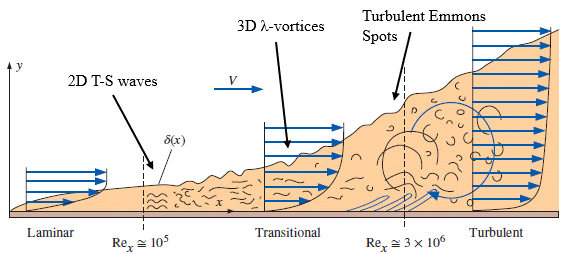
\includegraphics[width=0.70\linewidth]{pictures/flat_plate_transition_annotated_2.png}
    \caption{Transition process from a laminar to a turbulent boundary layer over a flat plate, showing the formation of T-S waves, $\lambda$-vortices and Turbulent Emmons spots. Adapted from \cite{transition_picture}.}
    \label{fig:transition from laminar to turbulent over a flat plate}
\end{figure}

These $\lambda$-vorticies promote the mixing between higher velocity fluid in the freestream and the lower momentum fluid nearer to the wall. As a result the velocity profile is unstable, which culminates in the stochastic appearance of high-frequency turbulent Emmons spots \cite{emmons1951spots}. As these spots move, they coalesce and form an arrowhead geometry as in \Cref{fig:single_turbulent_spot}. They expand at a wedge angle of approximately $8^\circ$ to $12^\circ$ \cite{hu2025experimental}. The leading edge is convected downstream at roughly $0.9 U_1$, while the trailing edge travels at $\approx 0.5 U_1$. \cite{bajpai2026turbulent}. At some point, they have fully merged to form a continuous, fully developed turbulent boundary layer.

\begin{figure}[H]
    \centering
    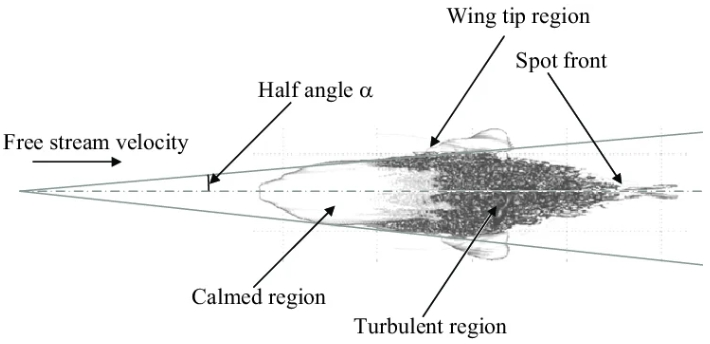
\includegraphics[width=0.7\linewidth]{pictures/arrowhead.jpeg}
    \caption{Single annotated turbulent spot and its arrowhead geometry. It will coalesce to form a fully turbulent boundary layer. From \cite{redford2012numerical}.}
    \label{fig:single_turbulent_spot}
\end{figure}

These values of wedge angle match closely what was found in \Cref{sec:turbulent wedge profile}. The experiment can also indirectly verify the slower trailing edge compared to the leading edge as the wedge angle was seen to increase with streamwise distance. In incompressible flow this is only possible if the leading edge is traveling more quickly than the trailing edge, effectively pushing the turbulent spot spanwise.

Transition can also be triggered by an adverse pressure gradient through a Laminar Separation Bubble (LSB). If the laminar boundary layer lacks sufficient momentum to overcome the rising pressure, it undergoes laminar separation. As shown in \Cref{fig:LSB sketch}, the resulting detached shear layer is highly unstable. Turbulent fluctuations amplify more rapidly in the separated flow as it is further from the wall, and this enhances momentum exchange with the freestream. This increased kinetic energy allows the flow to overcome the pressure gradient and reattach to the surface, creating a Laminar Separation Bubble \cite{schlichting1961boundary}. In other words, transition is triggered by flow separation and is necessary for LSBs to occur. The location of the transition point and the LSB is highly sensitive to the pressure distribution around the streamlined body. Adverse pressure gradients will reduce the distance required for flow to separate and for T-S waves to breakdown into turbulence, whereas favorable pressure gradients will help stabilize the laminar flow, making it harder for separation and LSBs to form.

\begin{figure}[H]
    \centering
    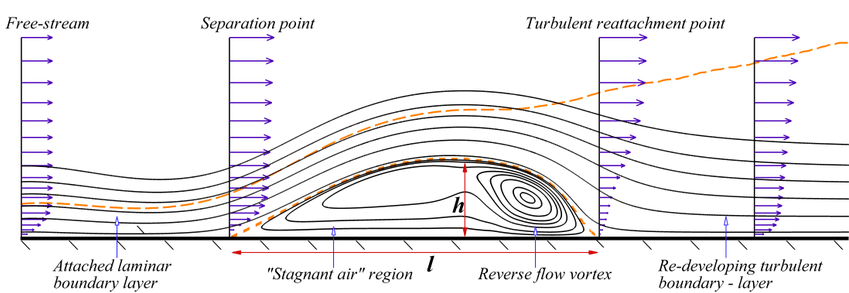
\includegraphics[width=0.75\linewidth]{pictures/laminar_separation_bubble.png}
    \caption{Formation of a Laminar Separation Bubble from the reattachment of turbulent flow after its transition from prior separated laminar flow. From \cite{LSB_picture}.}
    \label{fig:LSB sketch}
\end{figure}


\subsection{Practical uses of the high sensitivity of boundary layers to small surface imperfections}

Many industries (such as the aerospace, motorsport, turbomachinery, naval industries) are heavily impacted by the laminar to turbulent transition of boundary layers around different objects. It's high sensitivity to very small surface imperfections can make it very hard for engineers to avoid transition and lower skin-friction drag, but can also be useful to avoid flow separation and decrease pressure drag.

For example, it is often useful to have fully turbulent flow early on when designing an aeroplane wing. Lift-producing aerofoils must have an APG on its suction surface aft of its suction peak point. If the boundary layer lacks sufficient kinetic energy to overcome the rising pressure, the flow detaches, leading to a loss of lift called stall.

Turbulent boundary layers are inherently more resilient to APG-induced separation due to the momentum exchange between the high-velocity freestream and the near-wall region. Consequently, it is often advantageous to force the flow into a turbulent state prior to the region of maximum APG. As shown in \Cref{fig:flow control devices}, the implementation of passive flow control devices, such as tripwires or vortex generators, intentionally induces turbulence. This ensures the boundary layer remains attached at higher angles of attack, and increases safety in low-speed conditions.


\begin{figure}[H]
\centering
\begin{minipage}{0.49\textwidth}
    \centering
    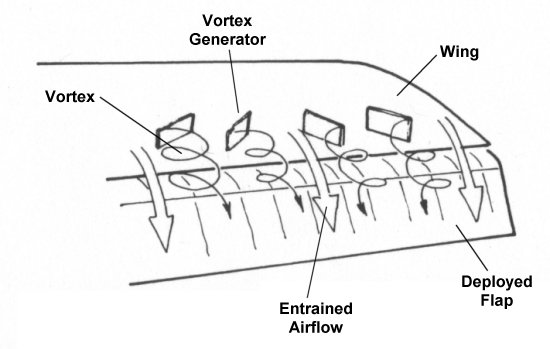
\includegraphics[width=0.86\linewidth]{pictures/vortex_generator.jpg}
    \caption{Sketch of a vortex generator on the suction surface of the wing of an aircraft. This induces turbulence and helps the flow stay attached on the lift-producing deployed flap. From \cite{aerospaceweb_vortex}.}
    \label{fig:flow control devices}
\end{minipage}
\hfill
\begin{minipage}{0.49\textwidth}
    \centering
    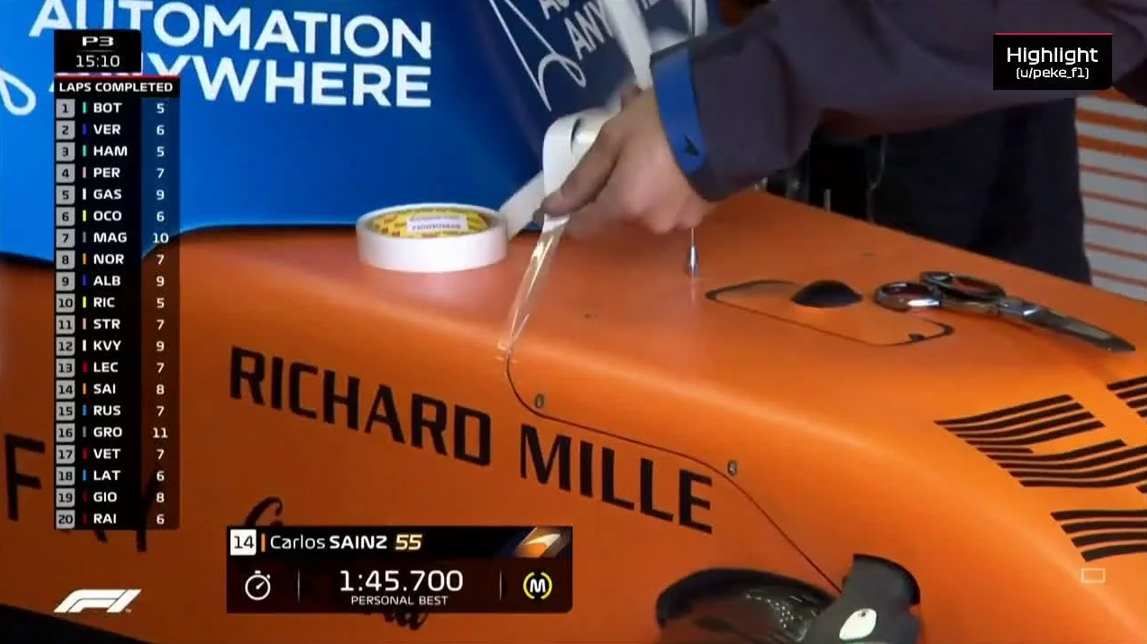
\includegraphics[width=0.98\linewidth]{pictures/F1_car_tape_2.png}
    \caption{McLaren F1 mechanic taping up small gaps between the carbon panels on the front of car's chassis to avoid early transition to turbulence and reduce skin-friction drag. From \cite{mclaren_f1_taping}.}
    \label{fig:F1 tape on gaps}
\end{minipage}
\end{figure}

While turbulence aids in keeping flow attached, it increases skin-friction drag due to the steeper velocity gradient at the wall and the higher wall shear stress $\tau_w$ compared to a laminar profile. For this reason, Formula One teams often tape up small gaps between their chassis components and have very strict surface roughness tolerances to delay the transition as much as possible. Cyclists and swimmers shave their body in part to reduce their skin friction coefficient $C_f$ as much as possible. Ice formation on planes or boats can also trigger premature transition, leading to a substantial increase in skin-friction drag and fuel consumption. This becomes even worse if imperfections become large enough to separate the flow entirely as this cause the formation of a turbulent wake and extra form drag.

The transition to turbulence can also produce thermal challenges. Turbulent boundary layers exhibit significantly higher convective heat transfer coefficients than laminar ones. Consequently, early transition will increase thermal loading on parts like rocket nozzles or hypersonic vehicles. Advanced coatings and very high-precision manufacturing can avoid early transition into turbulence and reduce thermal loading.


\section{Conclusions}

\begin{itemize}
    \item The Reynolds number at which flow on a smooth plate transitions from laminar to turbulent is greatly affected by surface disturbances such as roughness elements or trip wire. Depending on the type of surface disturbance, the transition will also be more or less sudden.
    \item If given enough distance, boundary layers will always transition to turbulent even when no disturbances are present.
    \item The horizontal transition between laminar and turbulent flow is relatively sudden and the intermittent wedge region $X_{trans}-X_{turb}$ is therefore quite narrow. The angle formed by the wake is not constant and increases with distance downstream of the initial trip.
    \item The size of eddies in turbulent flow is hard to measure due to its chaotic and stochastic nature, but an average can be roughly estimated by looking at frequency components in a hot-wire voltage signal.
    \item Boundary layer velocity profiles can be analyzed on a Clauser plot. The law of the wall can then be used to estimate the skin friction coefficient $C_f$ and the friction velocity $U_*$.
    \item Turbulent boundary layers have highest turbulence intensity near the wall surface which lead to large velocity fluctuations there. The magnitude of these disturbances decreases pretty linearly with height from the wall, until it becomes null at the boundary layer surface.
\end{itemize}

\hl{Make a paragraph and add FTR conclusions}

\newpage
\bibliography{references}

\newpara
\newpara
\newpara
Unless stated otherwise, all Figures are from author.

\section{Appendix}
\appendix

\section{Nomenclature}
\Crefname{section}{Appendix}{Appendices}
\label{app:symbols}

This appendix provides a summary of the symbols, descriptions, and abbreviations used throughout this report.

\begin{table}[H]
    \centering
    \begin{tabularx}{\textwidth}{l X l l}
        \toprule
        \textbf{Symbol} & \textbf{Description} & \textbf{Value} & \textbf{Units} \\
        \midrule
        \textbf{Scalars (in $\mathbb{R}$})   &                                     &          &                             \\
        $\bar{u}$          & 10 \unit{\second} mean of the local flow velocity measured by the probe.                         &          & \unit{\metre \per \second} \\
        $\bar{U}_1$          & Mean of the freestream flow velocity.       &          & \unit{\metre \per \second} \\
        $u'$               & Root mean square (RMS) of the local flow velocity measured by the probe.                 &      & \unit{\metre \per \second}  \\
        $\lambda$               & Average length of a turbulent eddy.                       &     & \unit{\metre}            \\
        $N$             & Number of turbulent eddies.  &     &             \\
        $\mu$             & Dynamic viscosity of the air.  & 1.82 $\times 10^{-5}$    & \unit{\pascal \second}            \\
        $\rho$             & Density of the air.  & 1.225    & \unit{\kilogram \per \metre \cubed}          \\
        $L$             & Distance between the leading edge of the plate and the probe.  & 1.14    & \unit{\metre}          \\
        $Re_x$           & Reynolds number of the flow based on distance from the leading edge of the plate.     & $\frac{\rho \bar{U}_1 L}{\mu}$   &             \\
        $\nu$             & Kinematic viscosity of the air.  & $\frac{\mu}{\rho}$    & \unit{\metre \squared \per \second}            \\
        $y$          & Vertical distance between the probe and the surface of the plate.                         &          & \unit{\metre} \\
        $\delta$          & Thickness of the boundary layer (assume 99\% thickness).                         &          & \unit{\metre}  \\
        $x$          & Streamwise distance from the leading edge of the plate.                      &          & \unit{\metre}  \\
        $\eta$          & Non-dimensional distance from the surface of the plate.                         &  $\frac{y}{\delta}$       &   \\
        $C_f$          & Skin friction coefficient.                         &          &  \\
        $U_*$          & Friction velocity.                         &          & \unit{\metre \per \second}  \\
        $\tau_w$          & Wall shear stress.                     &          & \unit{\newton \per \metre \squared}  \\
        $\delta^*$          & Displacement thickness of the boundary layer.                     &   $\int_{0}^{\infty} \left( 1 - \frac{u}{U_{\infty}} \right) dy$         & \unit{\metre}  \\
        $\theta$          & Momentum thickness of the boundary layer.                    & $\int_{0}^{\infty} \frac{u}{U_{\infty}} \left( 1 - \frac{u}{U_{\infty}} \right) \, dy$         & \unit{\metre}  \\
        $H$          & Shape factor of the boundary layer profile.                  &  $\frac{\delta^*}{\theta}$        &   \\
        $X_{turb}$          & Wedge angle of the turbulent wake.                        &          & \unit{\degree}  \\
        $X_{trans}$          & Wedge of the turbulent and intermittent wake.           &          & \unit{\degree}  \\
        $R^2$          & Coefficient of determination           &          &   \\
        % \addlinespace
        % \textbf{Vectors (in $\mathbb{R}^3$}) &                                     &          &                             \\
        % $\mathbf{F_n}$    & External force on the gyroscope/rotor assembly.         &          & \unit{\newton} (\unit{\kg \m \per \second \squared}) \\
        % $\mathbf{Q_n}$    & External couple on the gyroscope/rotor assembly.        &          & \unit{\newton \metre} (\unit{\kg \m \squared \per \second \squared}) \\
        % $(\mathbf{i, j, k})$ & Unit Cartesian coordinates fixed to the frame of reference (defined canonically).            &     & (\unit{\metre}, \unit{\metre}, \unit{\metre})        \\
        % \addlinespace
        % \textbf{Operators}                  &                                      &          &                             \\
        % $\norm{\mathbf{u}}$         & Norm of any vector $\mathbf{u}$ ($\equiv \sqrt{u_x^2+u_y^2+u_z^2}, \hspace{1em} \mathbb{R}^3 \to \mathbb{R}$).            &          &                            \\
        % $\dot{a}$         & Derivative of any scalar $a$ with respect to time ($\equiv \dv{}{t}$).            &          &                            \\

        \bottomrule
    \end{tabularx}
\end{table}

\section{Numerical Derivation of the Boundary Layer Parameters}
\Crefname{section}{Appendix}{Appendices}
\label{app:least squares method}

To determine the constants n and B for the power law and exponential velocity profiles, the models are linearized using logarithmic transformations to take the form $\mathbf{y} = \mathbf{X}\beta$. The optimal parameter $\beta^*$ is found by minimizing the sum of squared residuals, satisfying the Normal Equation:
\begin{equation*}
    \mathbf{X}^{T}\mathbf{X}\,\beta^* = \mathbf{X}^{T}\mathbf{y} \implies \beta^* = (\mathbf{X}^{T}\mathbf{X})^{-1}\mathbf{X}^{T}\mathbf{y}
\end{equation*}

Both the models used are single-parameter so $\mathbf{X}$ is a column vector of the independent variables $x_i(\eta_i)$ and $\mathbf{y}$ is the vector of dependent variables $y_i\bigg( \frac{\bar{u}}{U_1}_i\bigg)$.

\subsubsection{Power Law Model}

The power law model is in the form $\bar{u}/U_1=\eta^{1/n}$. Taking the natural logarithm linearizes the relationship:
\begin{equation*}
    \ln\left(\frac{\bar{u}}{U_1}\right) = \frac{1}{n} \ln(\eta)
\end{equation*}

$\mathbf{y}$ is therefore the log-velocity vector $y_i = \ln\bigg( \frac{\bar{u}}{U_1}_i\bigg)$ and the matrix $\mathbf{X}$ is in the form $x_i = \ln(\eta_i)$. Using the experimental data, solving for $\beta^*=1/n$ yields $\beta^*=0.154$. Therefore
\begin{equation*}
    n=\frac{1}{\beta^*}\approx 6.399
\end{equation*}

\subsubsection{Exponential Model}

The exponential model is in the form $\frac{\bar{u}}{U_1} = 1-e^{-B\eta}$. This is linearized as:
\begin{equation*}
    \ln\left(1 - \frac{\bar{u}}{U_1}\right) = -B\eta
\end{equation*}

Here, $\mathbf{y}$ is in the form $y_i = \ln\left(1 - \frac{\bar{u}}{U_1}_i\right)$ and $\mathbf{X}$ is $x_i = \eta_i$. Solving for $\beta^*=-B$ yields $\beta^*=4.6624$. Thus:
\begin{equation*}
    B = -\beta^* \approx 4.662
\end{equation*}

\end{document}
